\newpage
%
\subsection{Списание материалов}
\label{bp:MatOutput}

\subsubsection{Списание бумаги и картона}

Машинист гофроагрегата формирует потребность в сырье на основании задания на гофроагрегат.

Машинист гофроагрегата создает потребность в сырье, которую передает с водителем на склад материалов.
Кладовщик по заявке списывает сырье с помощью ТСД (рис. \ref{pic:d_TSD_1}). При этом кладовщик срезает этикетку с штрих-кодом с рулона для повторного контроля в конце смены.
В системе 1С:УПП ТСД создает документ ''Перемещение товаров''. В конце смены кладовщик в системе 1С:УПП проверяет созданный документ со срезанными ярлыками с штрих-кодом и проводит документ.


Кладовщик пишет отчет по остаткам в таблице MS Excel (рис. \ref{pic:d24}), учитывает рулоны по весу.
Факт списания сырья кладовщик также учитывает в файле Excel  (рис. \ref{pic:d24}).

В гофроагрегате на подаче на ''мокрой'' части на подаче сырья есть система учета сырья в системе Syncro, но он не подключен и не используется.
Подача сырья на гофроагрегат автоматизирована с помощи системы Newkuani (рис. \ref{pic:d_Newkuani}).

На момент проведения обследования система не запущена и находится в нерабочем состоянии (рис. \ref{pic:d_Newkuani_2}, \ref{pic:d_Newkuani_3}, \ref{pic:d_Newkuani_4}, \ref{pic:d_Newkuani_5}, \ref{pic:d_Newkuani_6}, \ref{pic:d_Newkuani_7}).

Возвраты сырья (рулоны бумаги и картона) с гофроагрегата не выполняются. Все сырье, перемещенное на гофроагрегат, считается списанным, хотя у гофроагрегата находятся остатки рулонов (рис. \ref{pic:d_Stock}). Недомоты не учитываются на складе.  
Забракованные рулоны в производстве тоже не возвращаются, а срабатываются.
В системе 1С:УПП настроен четкий учет сырья  по номерам рулонов.


Технолог производства создает расход сырья за сутки по нормативу в конце смены в таблице Excel и передает в бухгалтерию. Бухгалтер по материалам списывает сырье в системе 1С:Бухгалтерия расчетным путем по нормативам.
Полуфабрикаты на ГА не учитываются.





% Остатки в системе СБИС ведутся, но кладовщик не проверяет остатки в системе. Отчет формируется более 5 минут.
% По таблице \ref{pic:d38_1} кладовщик определяет остатки по сырью и передает инрис.цию машинисту гофроагрегата.
% Кладовщик в конце смены списывает рулоны бумаги и картона в форме MS Excel (рис. \ref{pic:d38_1}).
% По форме \ref{pic:d38} кладовщик записывает номера рулонов, которые были списаны в производство (рис. \ref{pic:d39}).
% В течение смены кладовщик списывает в системе СБИС рулоны в документ  “Накладная перемещения”.
% В системе СБИС кладовщик списывает рулон в метрах квадратных.


% По факту использования рулонов на гофроагрегате операторы на раскатах отмечают использованные рулоны в отчете по каждому раскату (рис. \ref{pic:d9}).
% В конце смены отчет с каждого раската мастер передает в БППП.
% Инженер-экономист в БППП на основании формы \ref{pic:d9} выполняет списание сырья в производство в системе СБИС.
% Инженер-экономист в БППП на основании формы \ref{pic:d9} создает отчет по браку (рис. \ref{pic:d10}) и передает в отдел ОТК.
% Брак считается по среднему.

% Инженер-экономист в БППП списывает рулоны в (рис. \ref{pic:d12}) в системе СБИС. 
% Инженер-экономист в БППП создает отчет по учету сырья (рис. \ref{pic:d13}) директору и начальнику производства.

\subsubsection{Учет вспомогательных материалов}

Списание по вспомогательным материалам происходит на основании устной заявки от бригадира. Кладовщик в системе 1С:УПП создает документ “Перемещение товаров” и оформляет списание вспомогательных материалов.

В бухгалтерии списание вспомогательных материалов дублируют в системе 1С:Бухгалтерия.

Списание поддонов выполняется по такой же схеме.



\subsubsection{Списание краски}

Списание краски происходит на основании устной заявки от бригадира. Кладовщик в системе 1С:УПП создает документ “Перемещение товаров” и оформляет списание вспомогательных материалов.

В бухгалтерии списание краски дублируют в системе 1С:Бухгалтерия.

% После использования краски машинисты взвешивают ведра с  остатками на весах (рис. \ref{pic:a14}) и на ведро машинист клеит ярлык с весом (рис. \ref{pic:a13}). Краска на каждой линии хранится на своем месте. Разбавленная краска не учитывается и остается в рабочих ведрах. 


% После взвешивания краски машинист пишет в документе ''Сменный рапорт машиниста'' количество использованной краски (рис. \ref{pic:a68}). На основании этих данных мастер смены ежедневно вносит данные для списания краски в системе 1С:УНФ.


% Краску списывает мастер в системе 1С:УНФ ежедневно на основании документа "Сменный рапорт машиниста", в который машинист вписывает руками количество израсходованной краски.  


% Списание вспомогательных материалов (клей, стрейч, скобы, ленты) выполняет мастер в конце месяца на основании данных инвентаризации и передает данные в бухгалтерию. Бухгалтер списывает  вспомогательных материалов в системе 1С:УНФ документом "Списание ТМЦ".
% % Хранение клея (11).

% Списание поддонов определяется по количеству переданных на склад. Учет поддонов выполняет мастер. Размеры поддонов определяются из упаковки.

% Раз в месяц мастер выполняет списание материалов (заготовки) и списание недопоставки от поставщика заготовки и списание на образцы (рис. \ref{pic:a74}, \ref{pic:a75}, \ref{pic:a76}). Все списания мастер сверяет с кладовщиком склада.

% \subsubsection{Списание бумаги и картона}

\begin{figure}
\begin{center}
  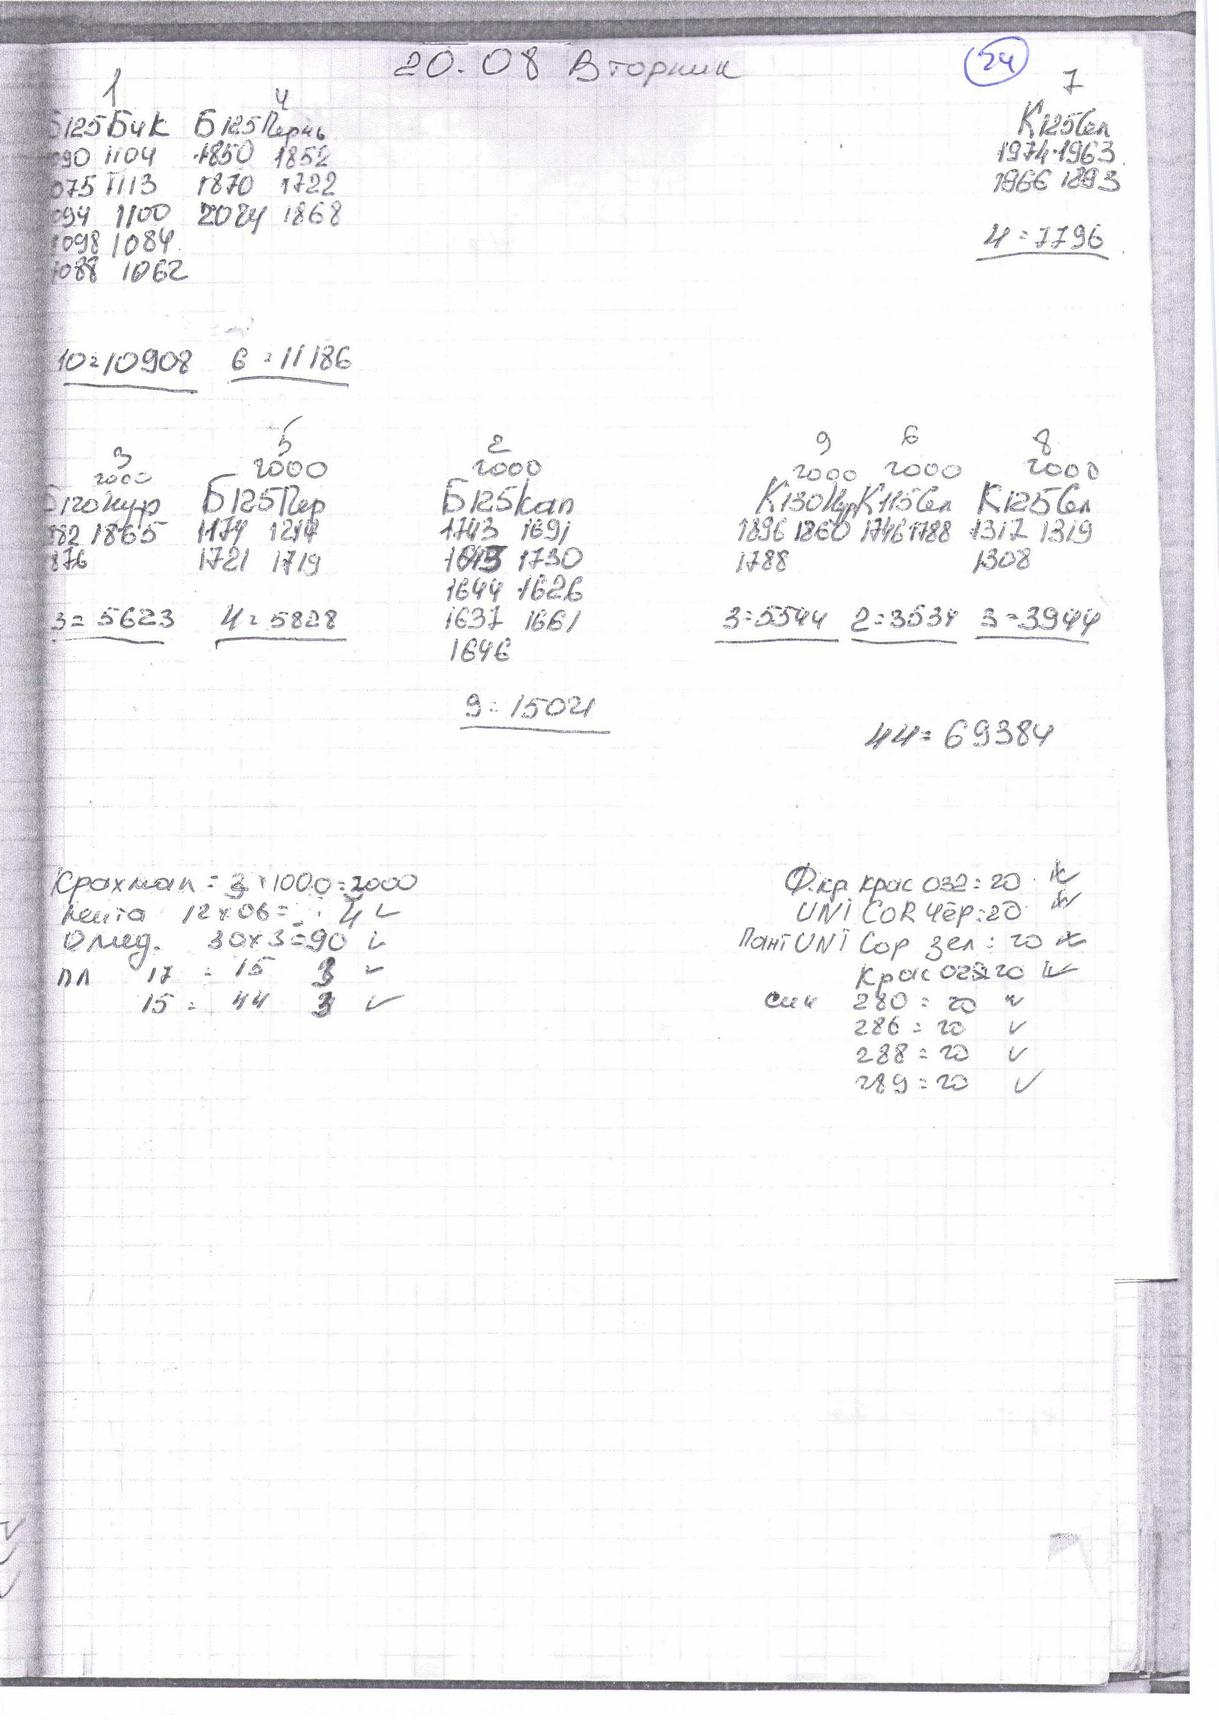
\includegraphics[height=0.8\textheight, width=\textwidth, keepaspectratio]{Pics/d24.jpg}
\end{center}
  \caption{Отчет по остаткам в таблице MS Excel}
  \label{pic:d24}
\end{figure}

\begin{figure}
\begin{center}
  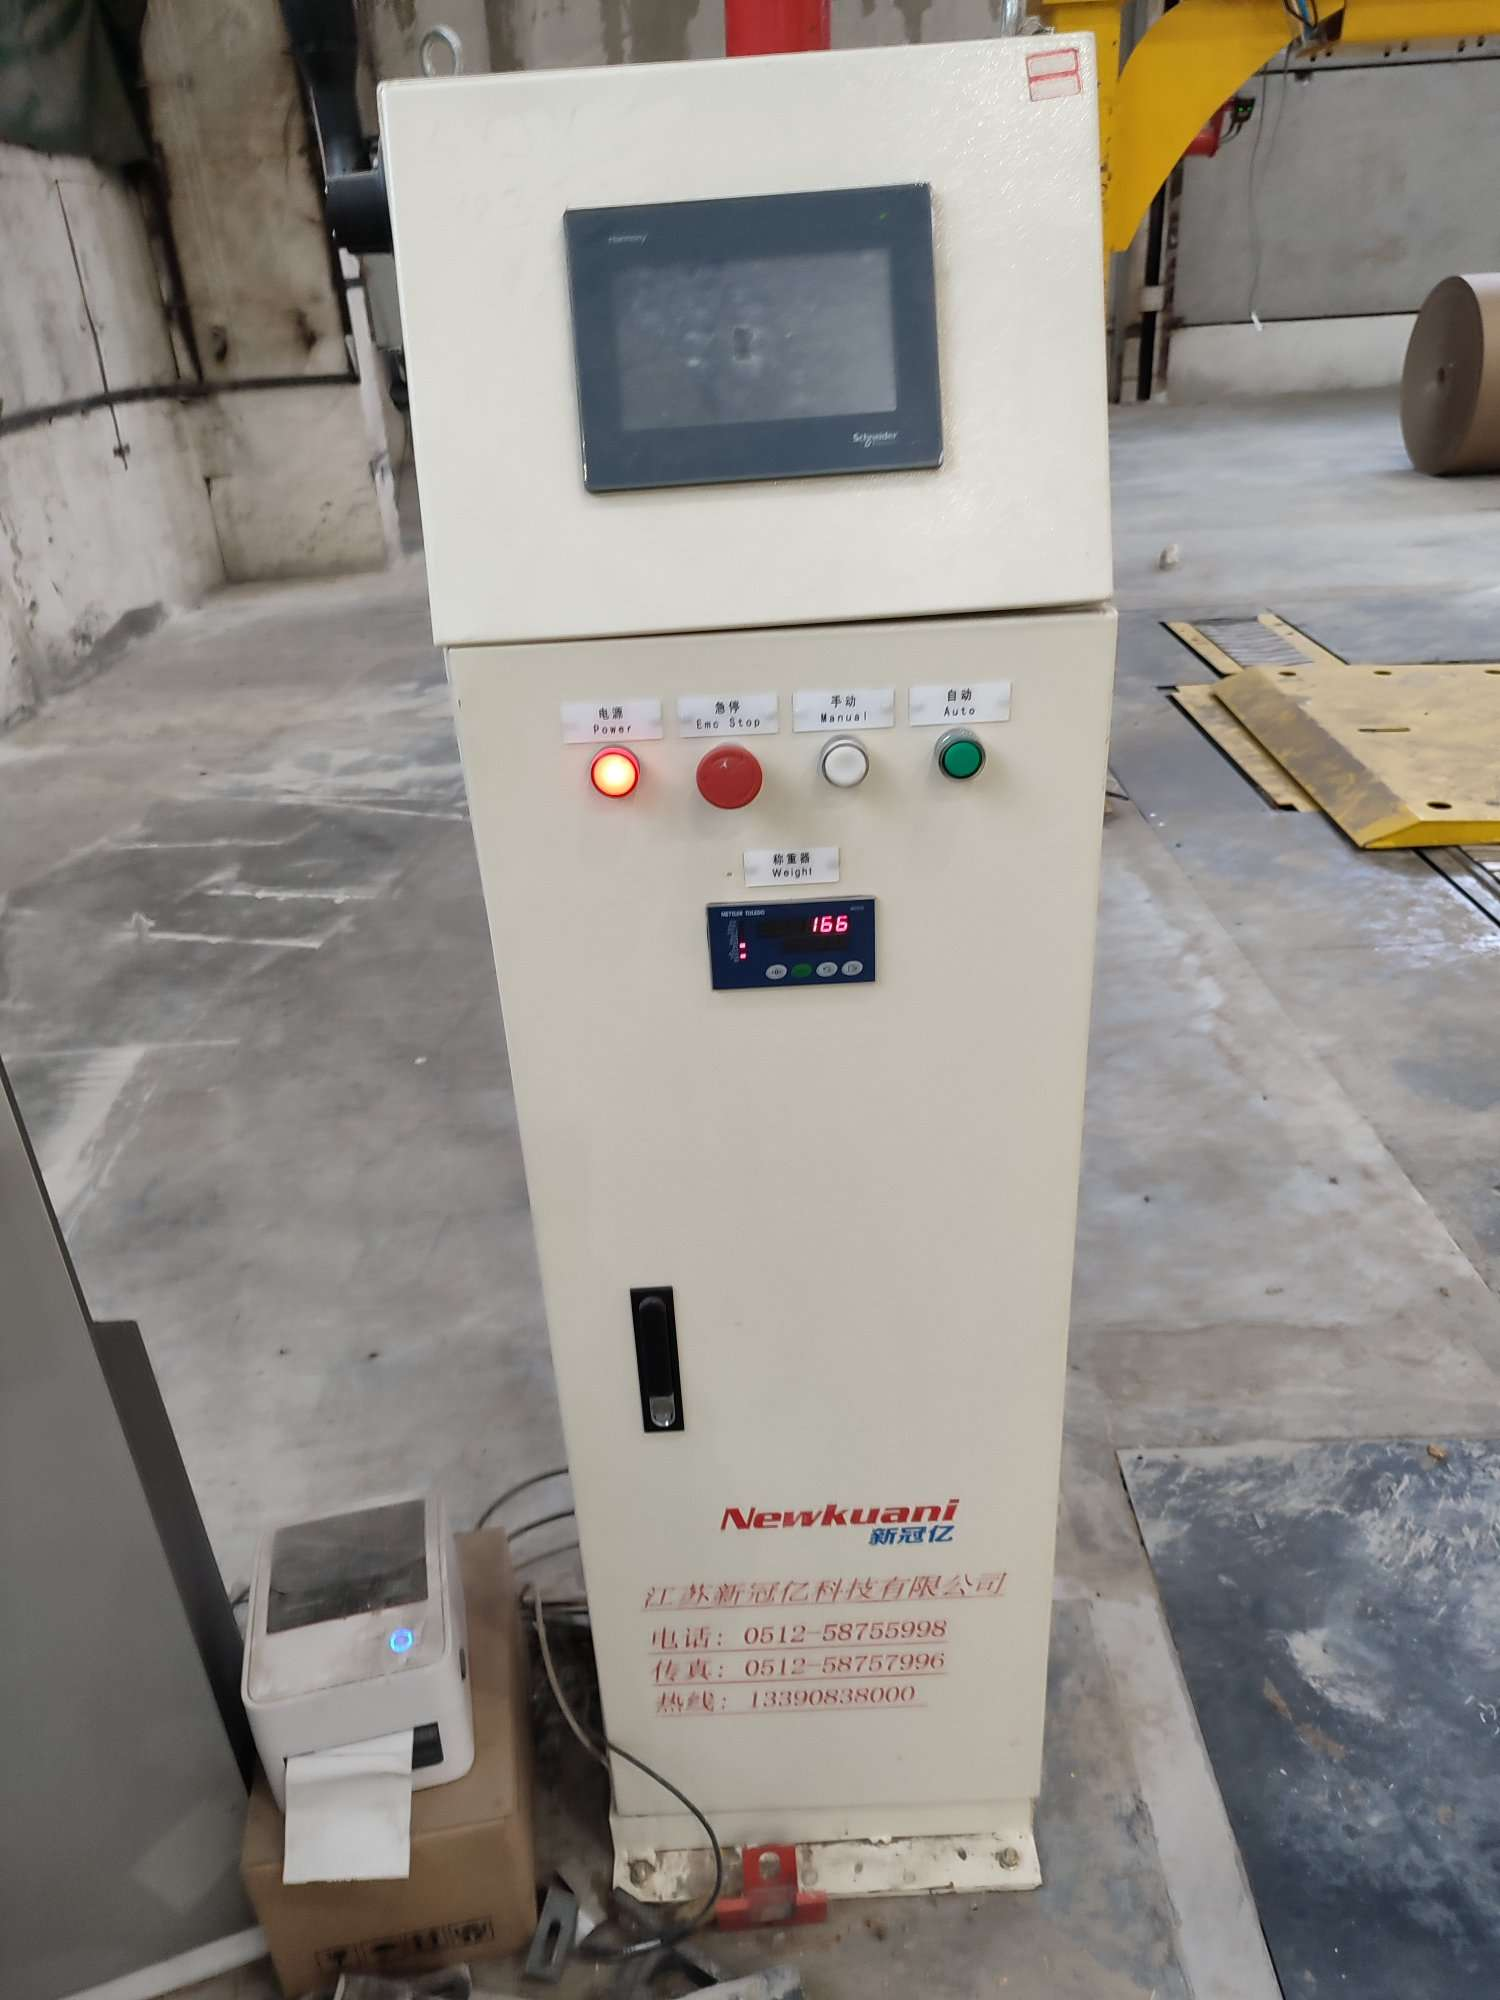
\includegraphics[height=0.4\textheight, width=\textwidth, keepaspectratio]{Pics/d_Newkuani.JPEG}
\end{center}
  \caption{Транспортная линия по сырью Newkuani}
  \label{pic:d_Newkuani}
\end{figure}

\begin{figure}
\begin{center}
  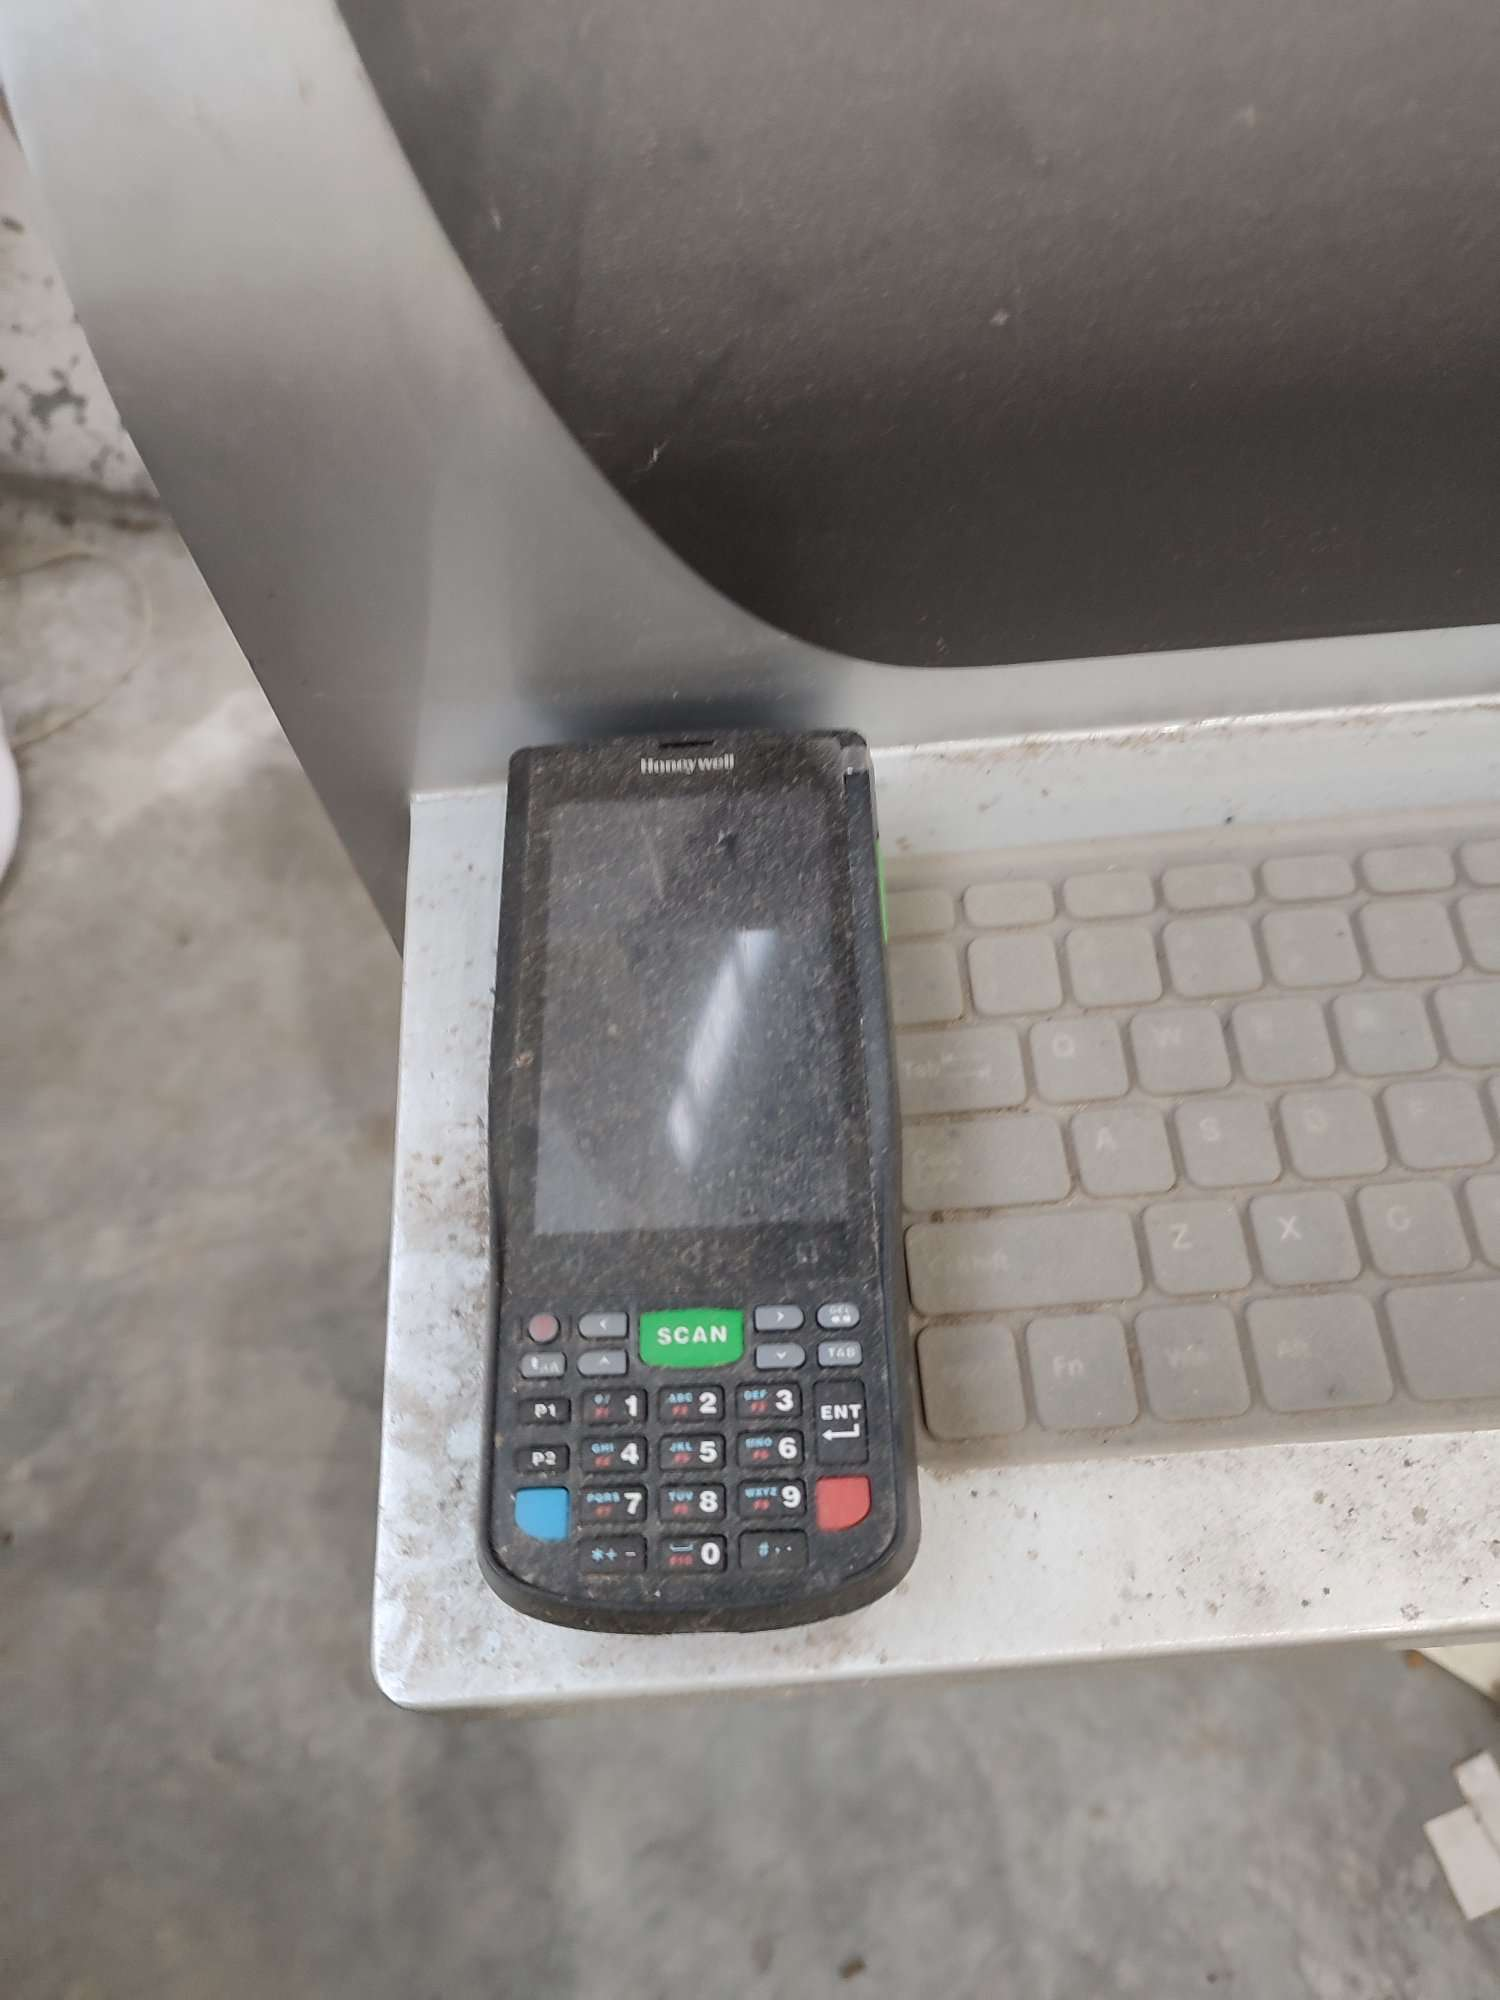
\includegraphics[height=0.4\textheight, width=\textwidth, keepaspectratio]{Pics/d_Newkuani_2.JPEG}
\end{center}
  \caption{Транспортная линия по сырью Newkuani}
  \label{pic:d_Newkuani_2}
\end{figure}

\begin{figure}
\begin{center}
  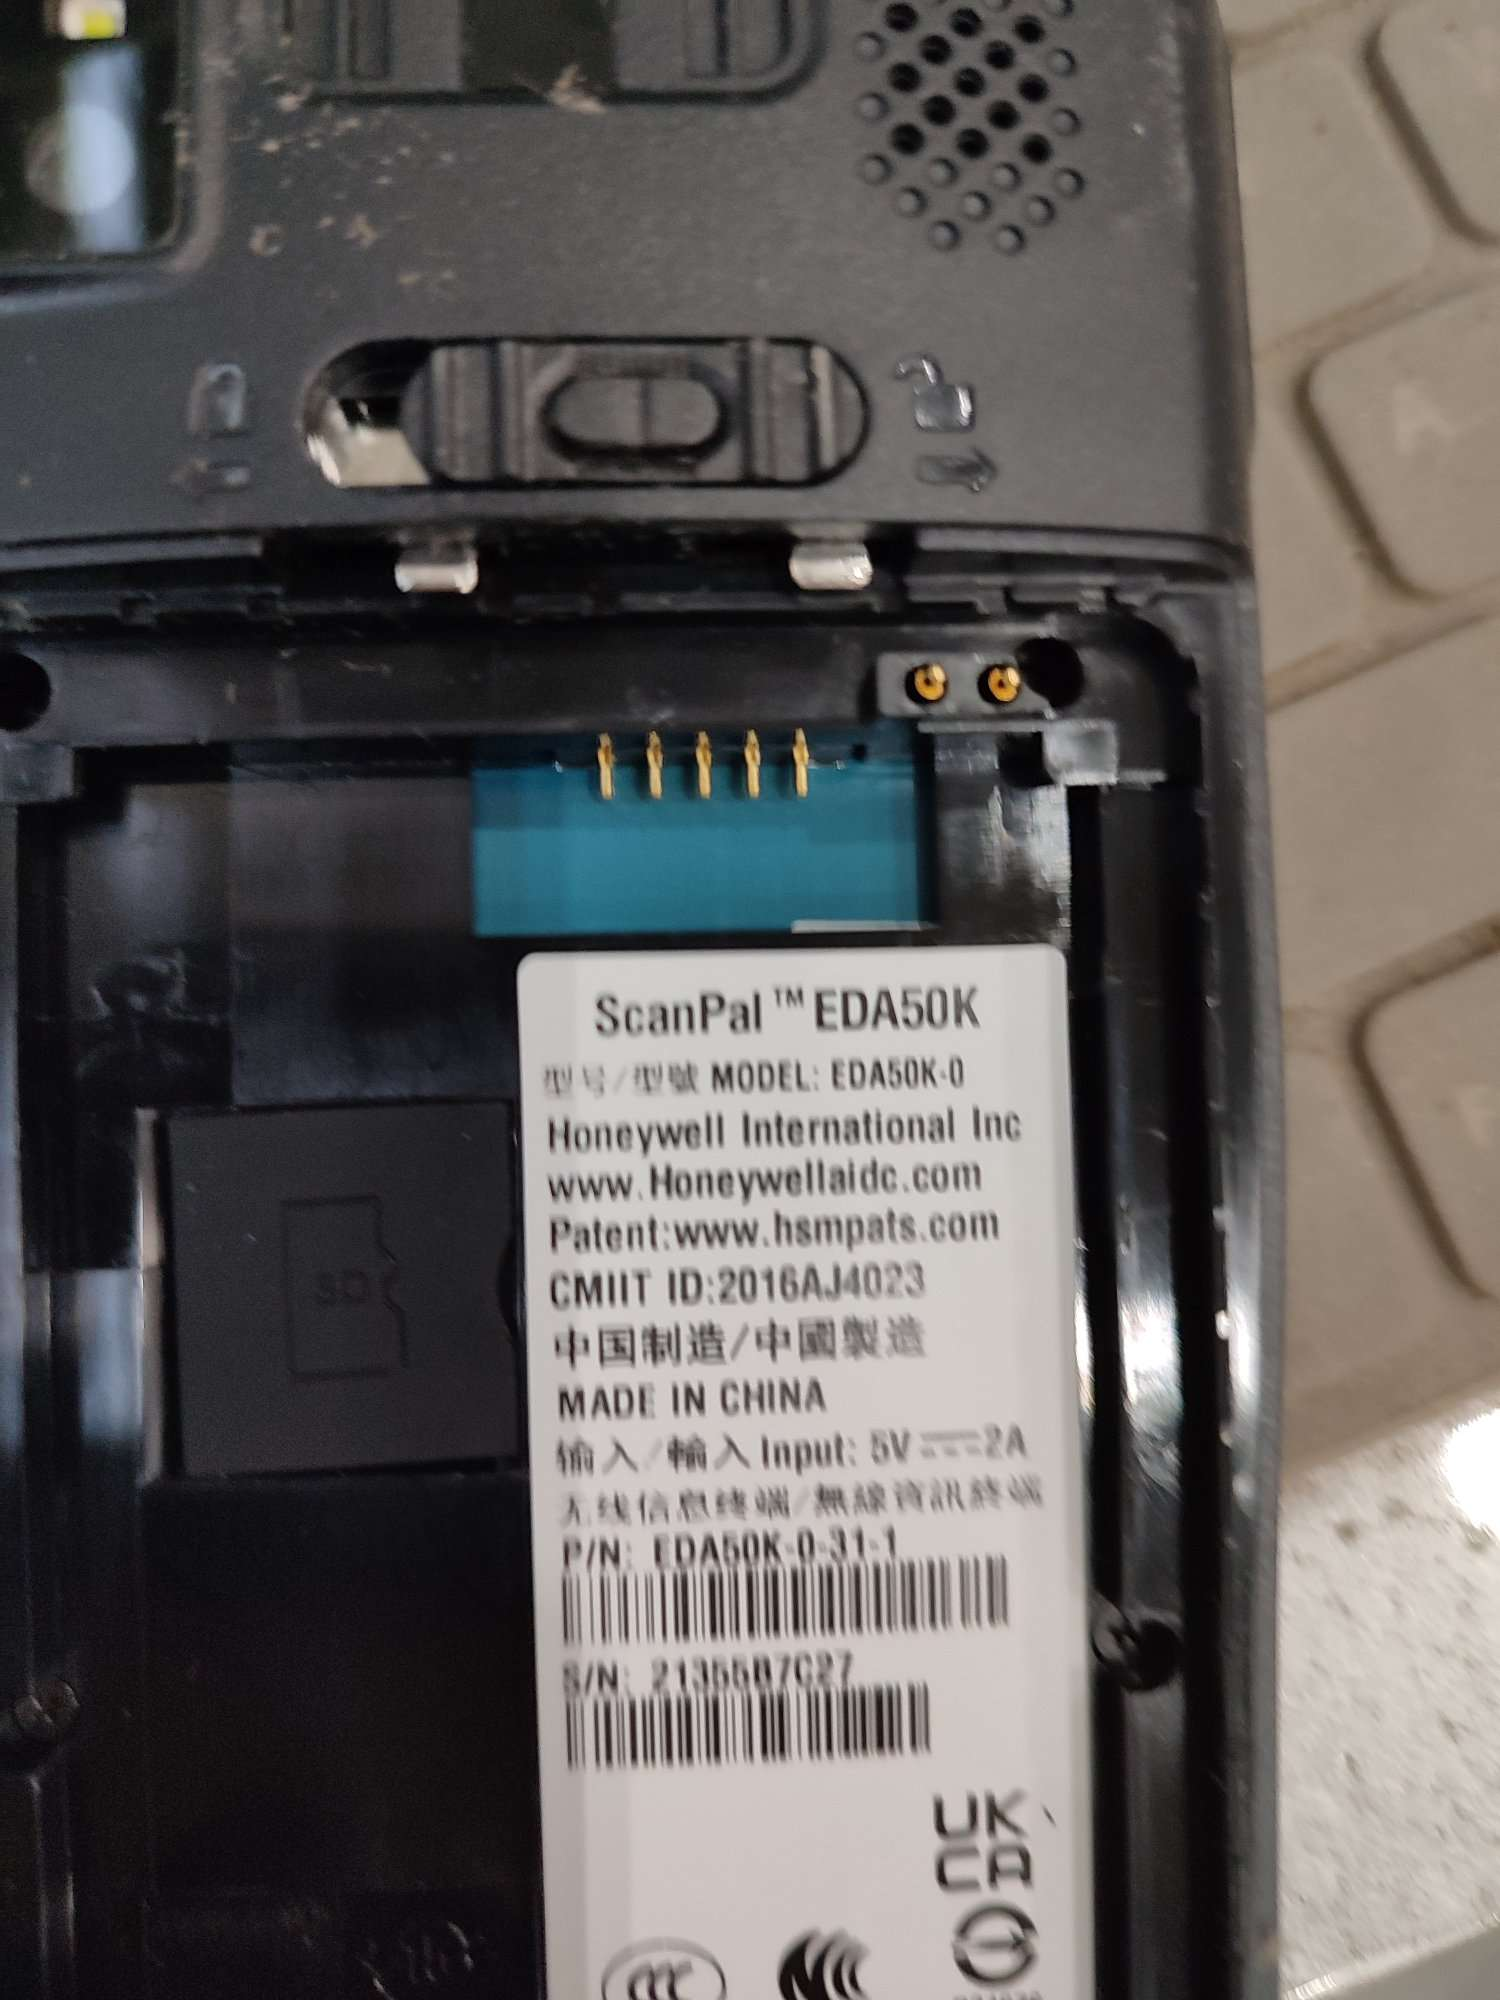
\includegraphics[height=0.4\textheight, width=\textwidth, keepaspectratio]{Pics/d_Newkuani_3.JPEG}
\end{center}
  \caption{Транспортная линия по сырью Newkuani}
  \label{pic:d_Newkuani_3}
\end{figure}

\begin{figure}
\begin{center}
  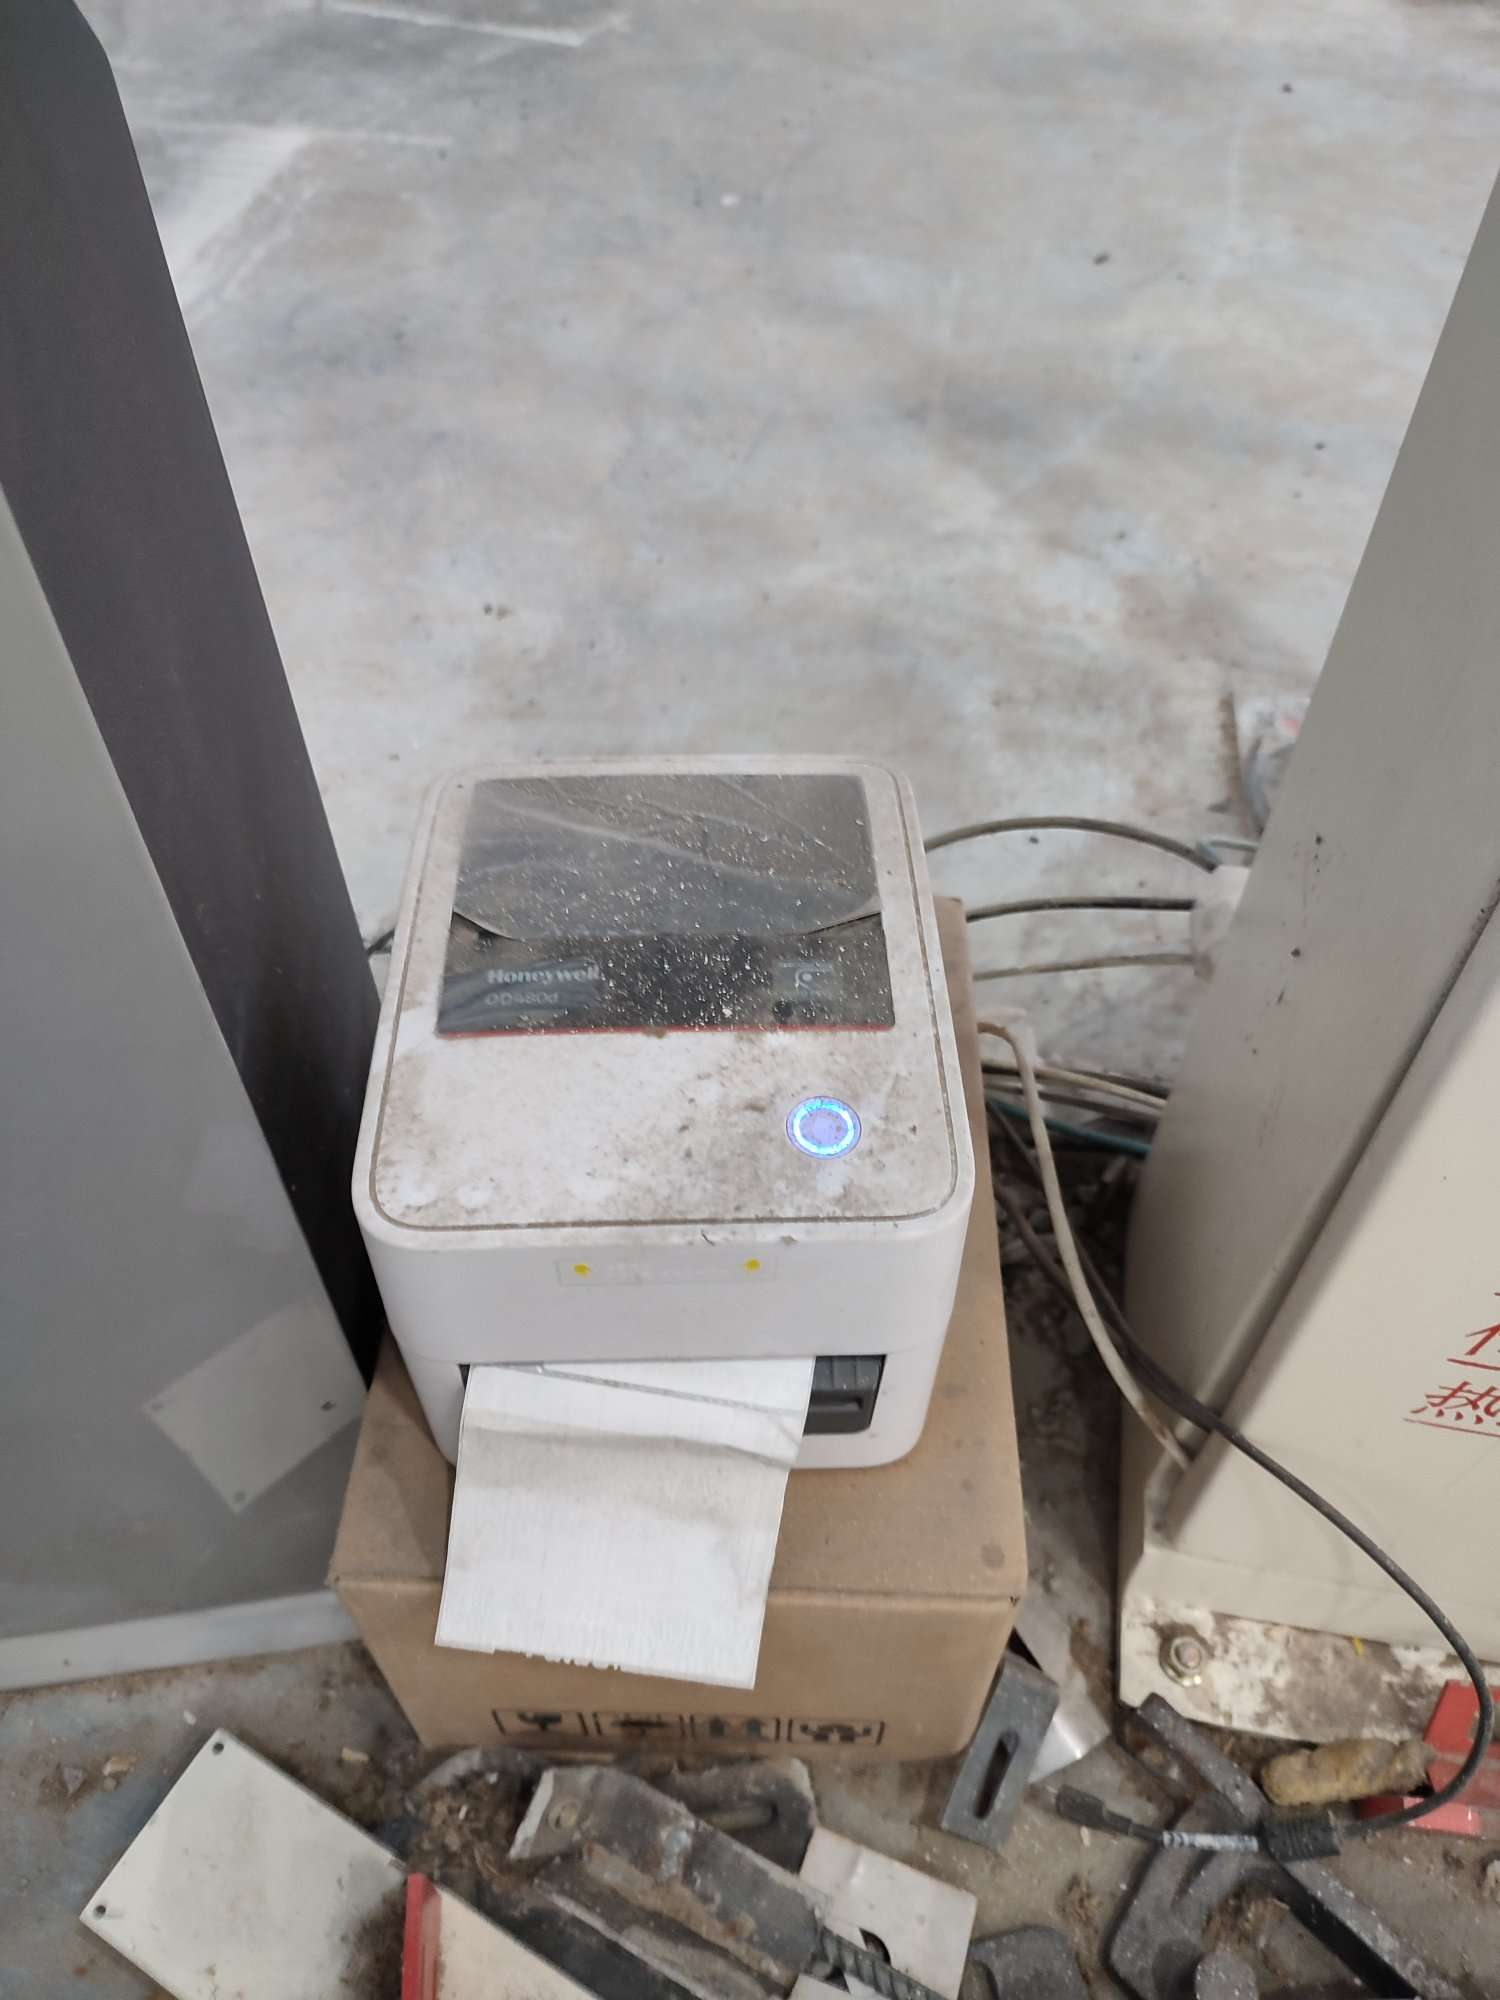
\includegraphics[height=0.4\textheight, width=\textwidth, keepaspectratio]{Pics/d_Newkuani_4.JPEG}
\end{center}
  \caption{Транспортная линия по сырью Newkuani}
  \label{pic:d_Newkuani_4}
\end{figure}

\begin{figure}
\begin{center}
  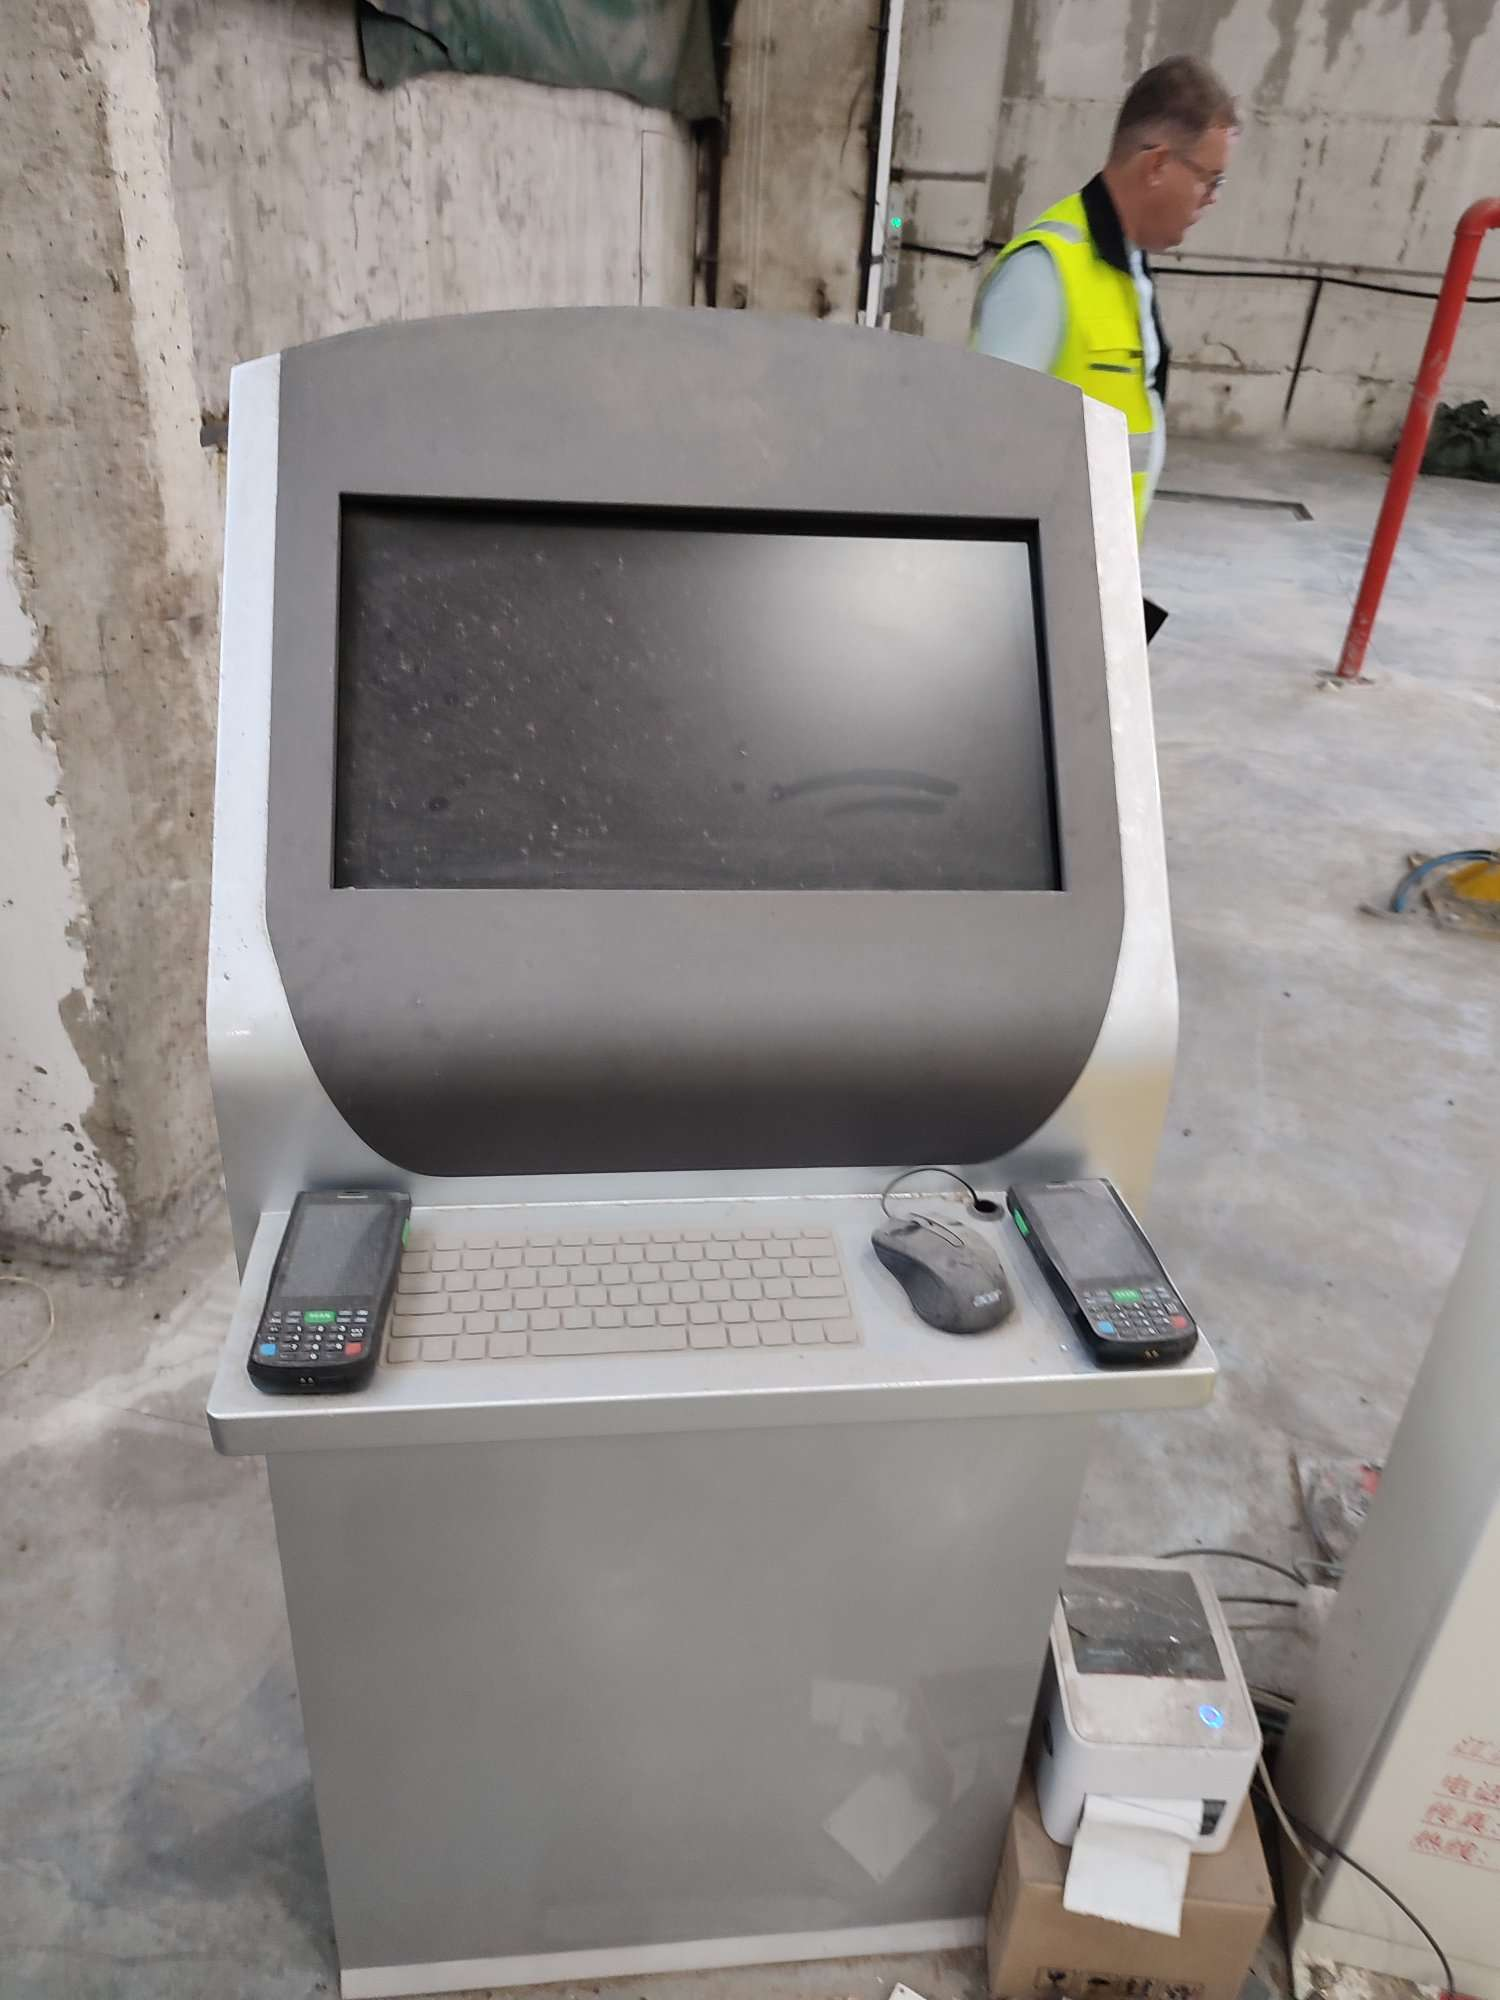
\includegraphics[height=0.4\textheight, width=\textwidth, keepaspectratio]{Pics/d_Newkuani_5.JPEG}
\end{center}
  \caption{Транспортная линия по сырью Newkuani}
  \label{pic:d_Newkuani_5}
\end{figure}

\begin{figure}
\begin{center}
  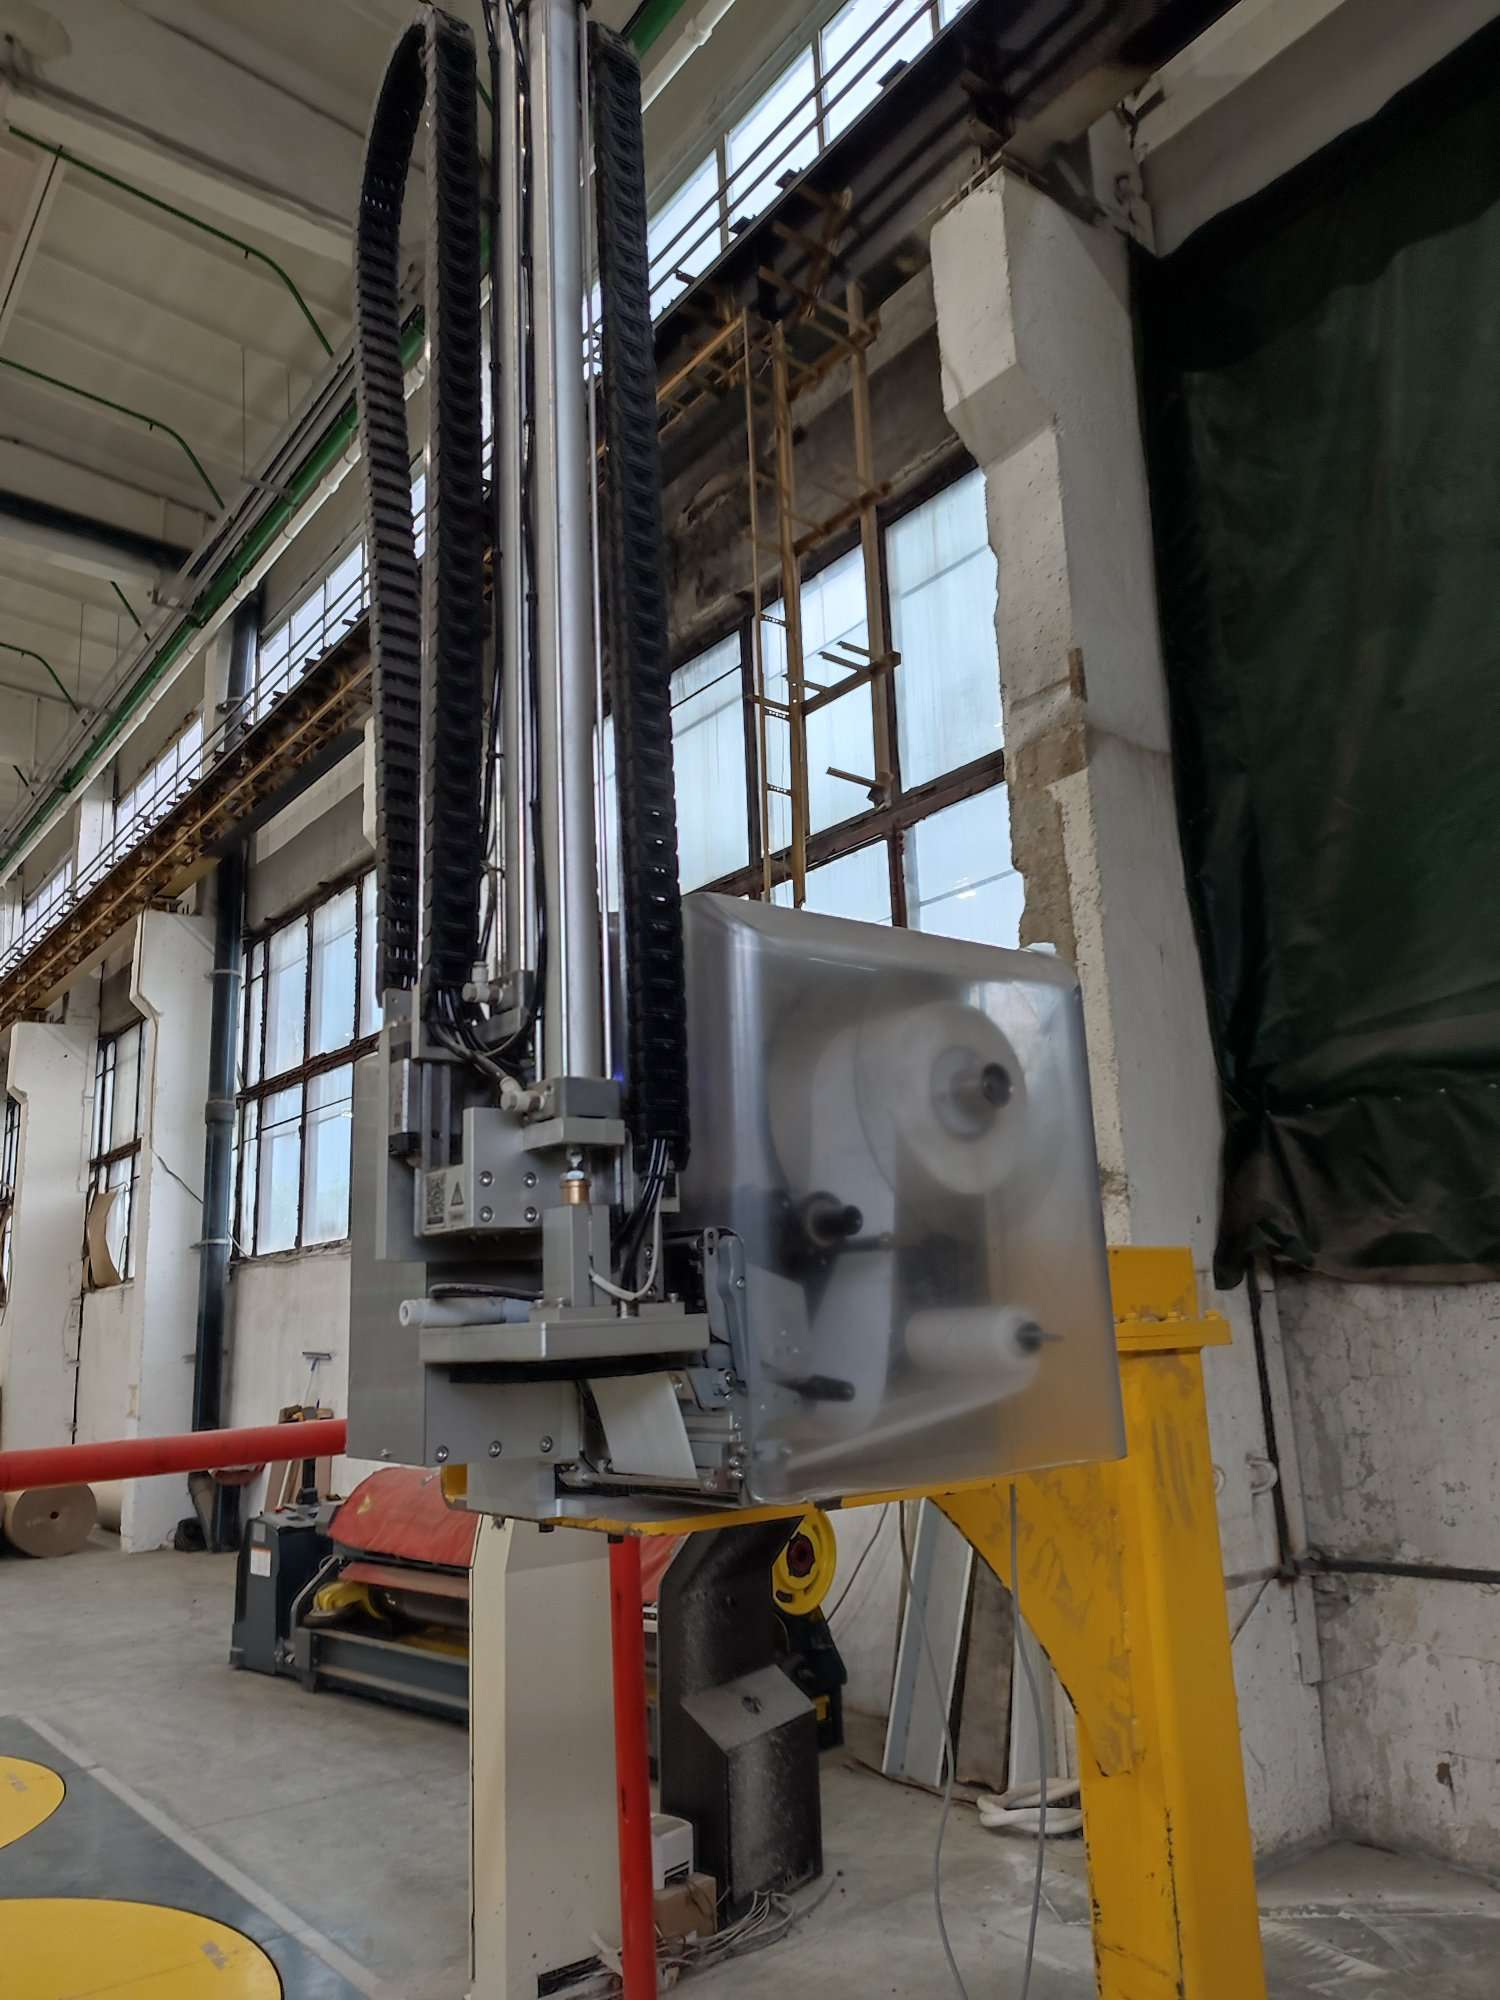
\includegraphics[height=0.4\textheight, width=\textwidth, keepaspectratio]{Pics/d_Newkuani_6.JPEG}
\end{center}
  \caption{Транспортная линия по сырью Newkuani}
  \label{pic:d_Newkuani_6}
\end{figure}

\begin{figure}
\begin{center}
  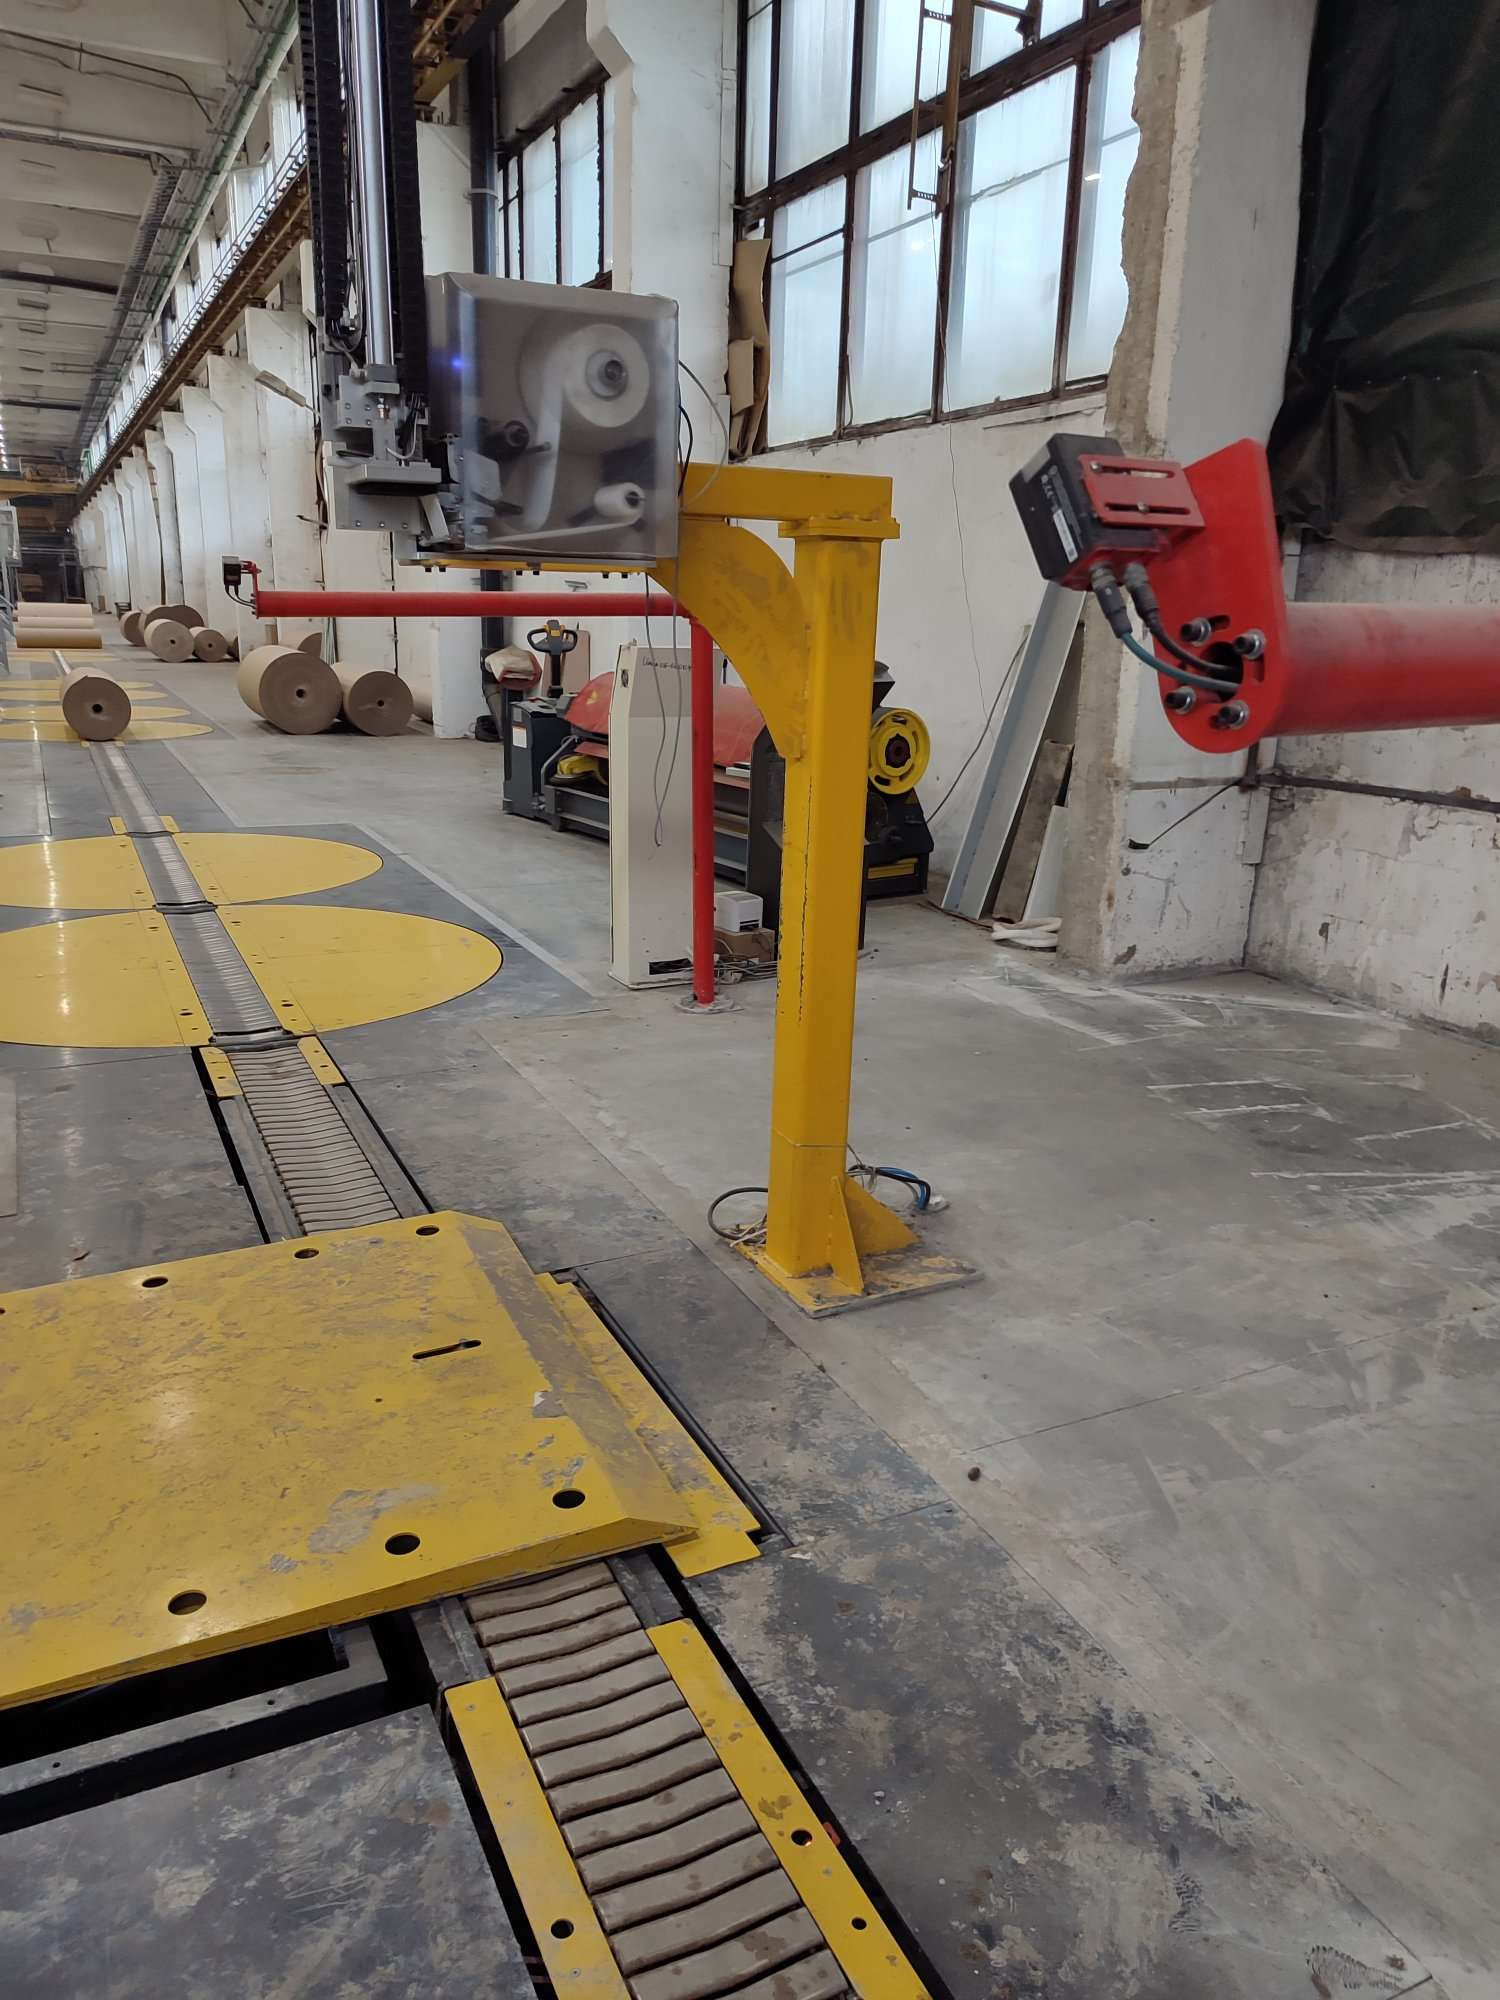
\includegraphics[height=0.4\textheight, width=\textwidth, keepaspectratio]{Pics/d_Newkuani_7.JPEG}
\end{center}
  \caption{Транспортная линия по сырью Newkuani}
  \label{pic:d_Newkuani_7}
\end{figure}

\begin{figure}
\begin{center}
  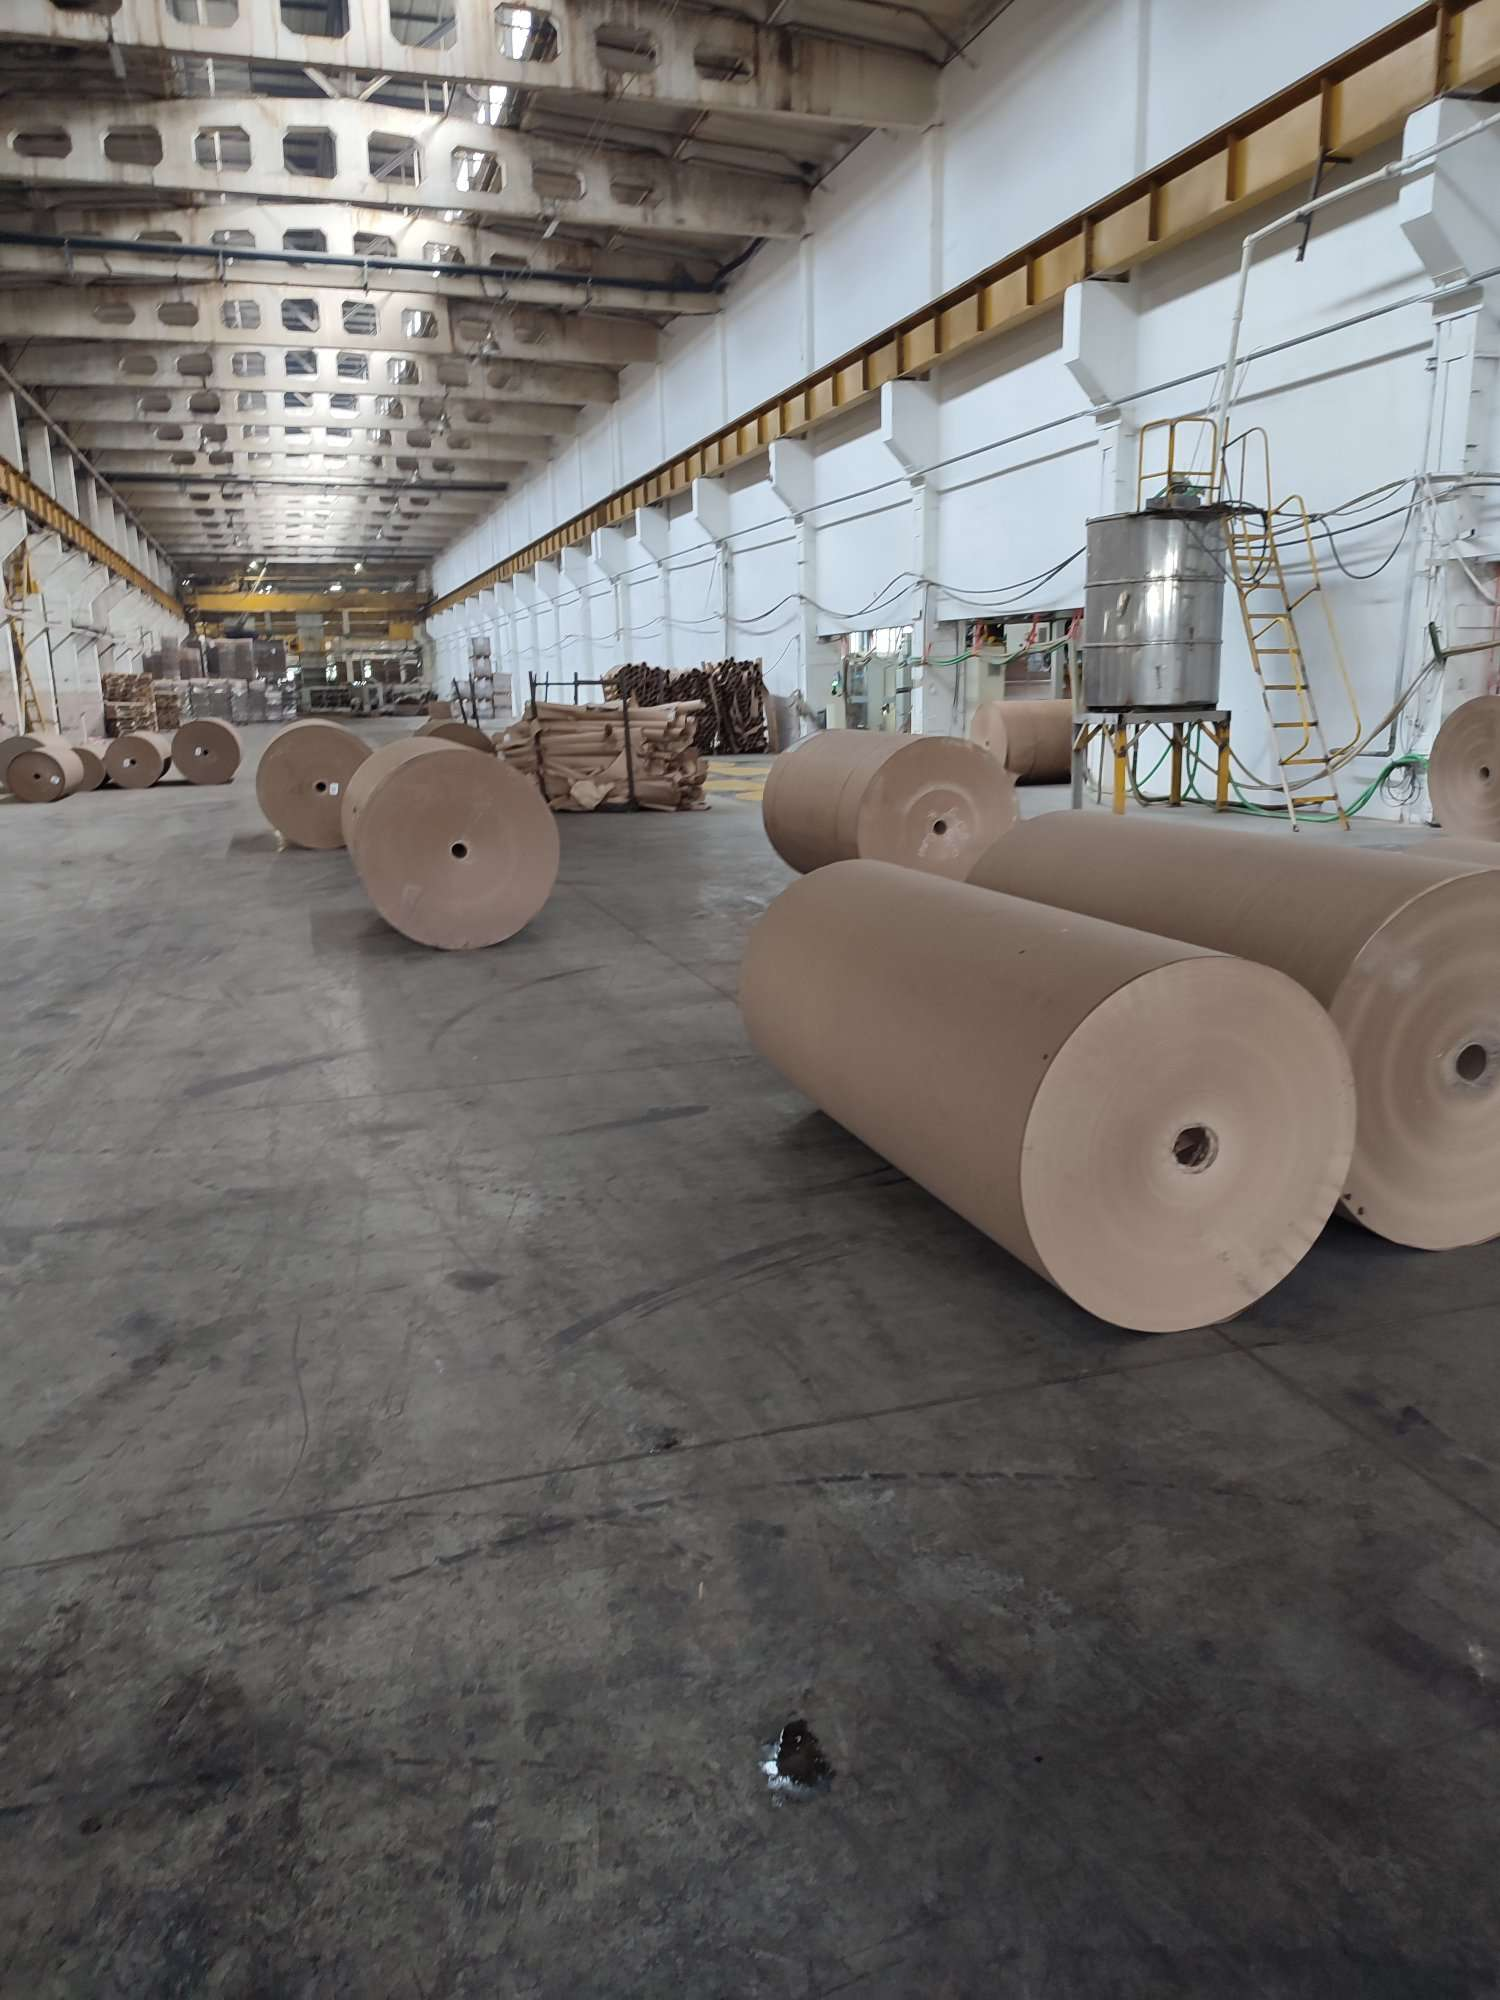
\includegraphics[height=0.8\textheight, width=\textwidth, keepaspectratio]{Pics/d_Stock.JPEG}
\end{center}
  \caption{Не полностью использованные рулоны у гофроагрегата}
  \label{pic:d_Stock}
\end{figure}

% \begin{figure}
% \begin{center}
%   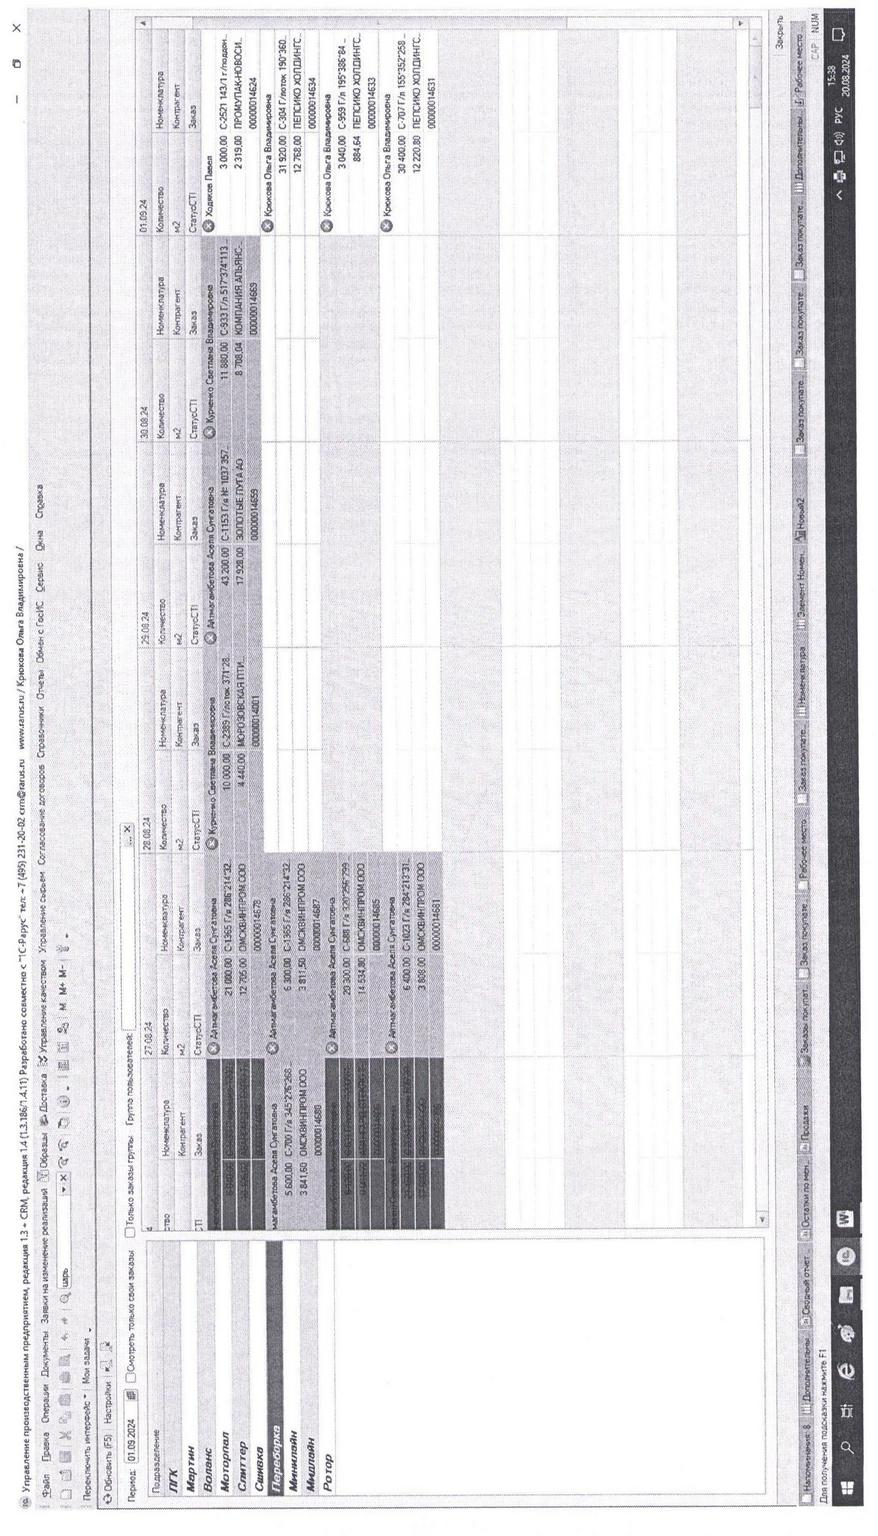
\includegraphics[height=0.94\textheight, width=\textwidth, keepaspectratio]{Pics/d10.jpg}
% \end{center}
%   \caption{Отчет по браку}
%   \label{pic:d10}
% \end{figure}

% \begin{figure}
% \begin{center}
%   \includegraphics[height=0.94\textheight, width=\textwidth, keepaspectratio]{Pics/d12.jpg}
% \end{center}
%   \caption{Списание рулонов со склада в СБИС}
%   \label{pic:d12}
% \end{figure}

% \begin{figure}
% \begin{center}
%   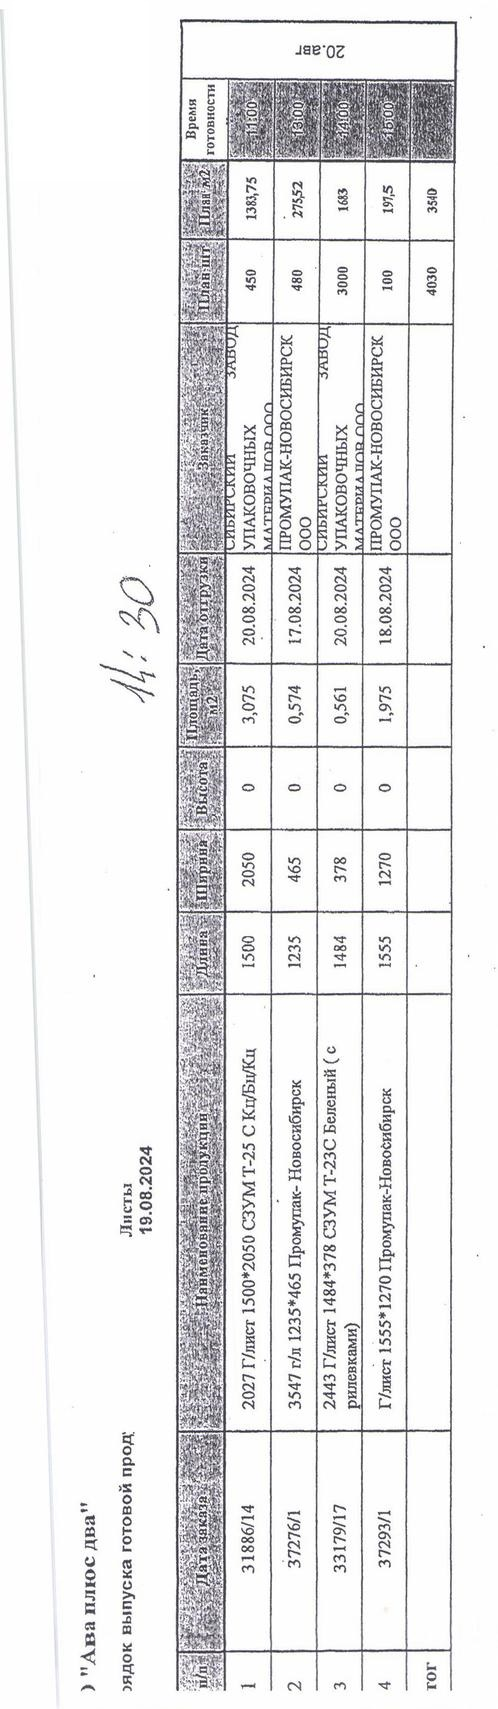
\includegraphics[height=0.8\textheight, width=\textwidth, keepaspectratio]{Pics/d13.jpg}
% \end{center}
%   \caption{Суточный отчет производства}
%   \label{pic:d13}
% \end{figure}

% \begin{figure}
% \begin{center}
%   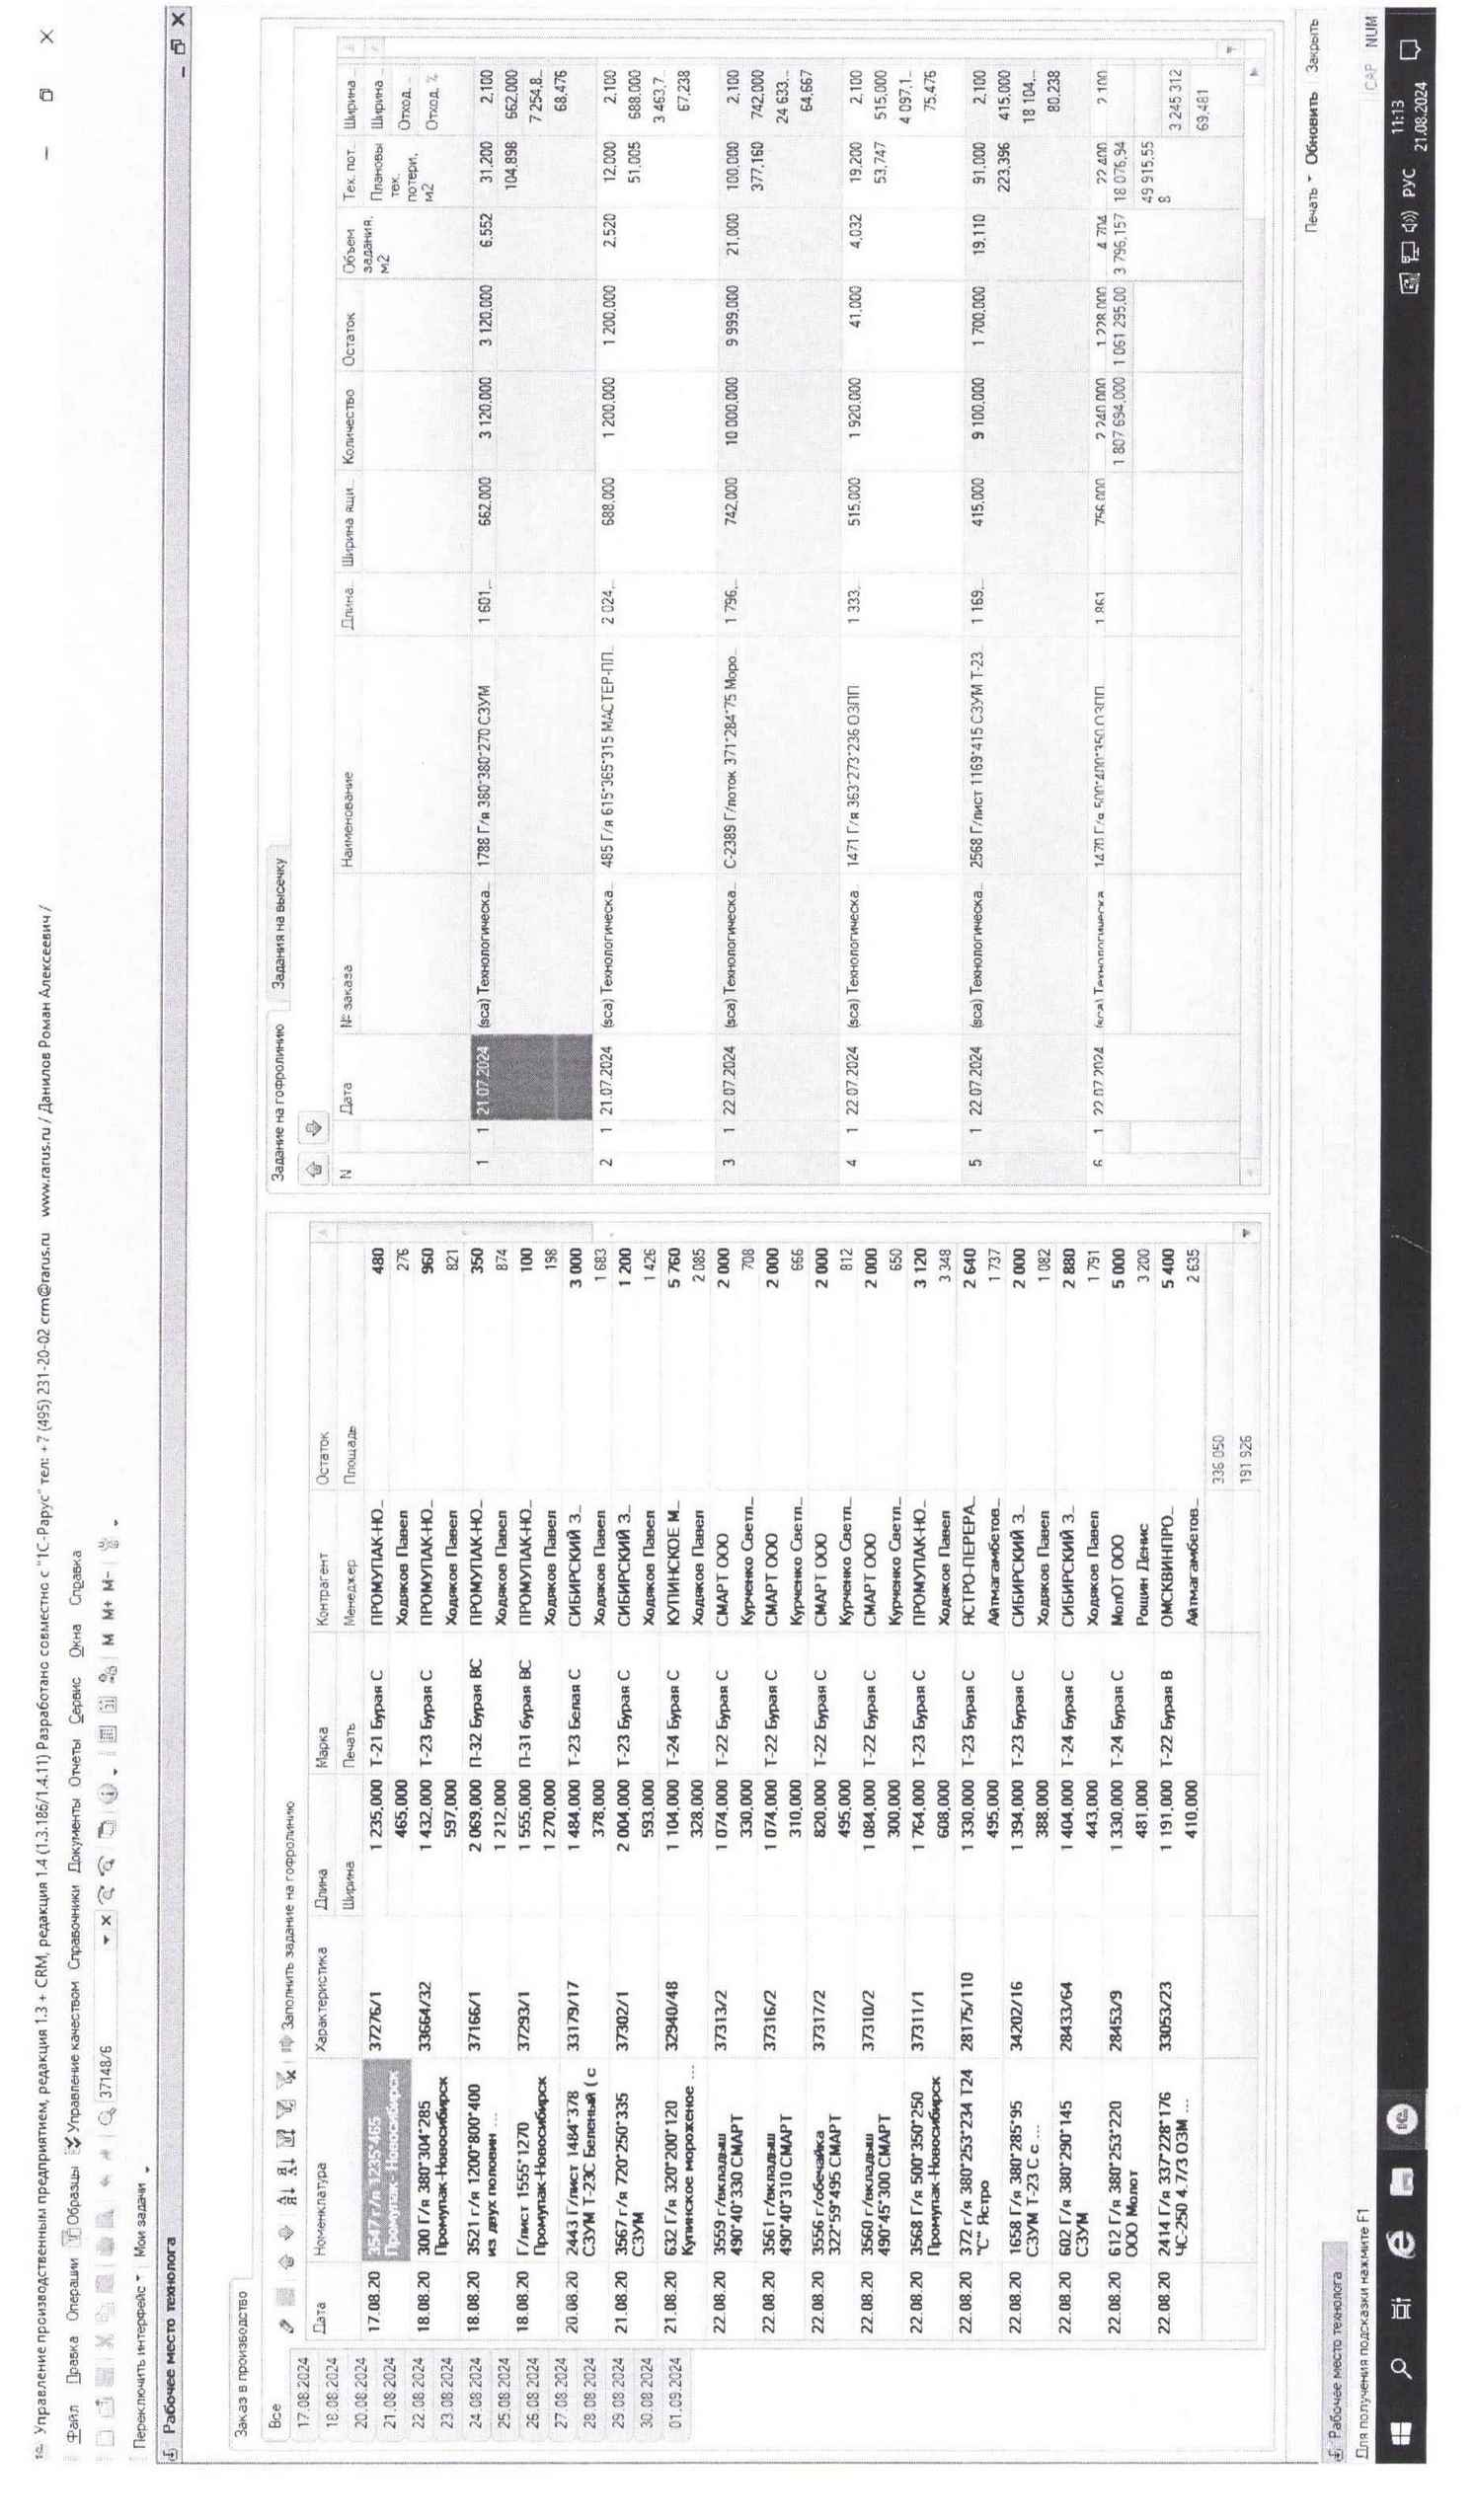
\includegraphics[height=0.8\textheight, width=\textwidth, keepaspectratio]{Pics/d18.jpg}
% \end{center}
%   \caption{Суточный расход по крахмалу}
%   \label{pic:d18}
% \end{figure}

% \begin{figure}
% \begin{center}
%   \includegraphics[height=0.8\textheight, width=\textwidth, keepaspectratio]{Pics/d17_1.jpg}
% \end{center}
%   \caption{Суточный расход по прочим материалам}
%   \label{pic:d17_1}
% \end{figure}

% \begin{figure}
% \begin{center}
%   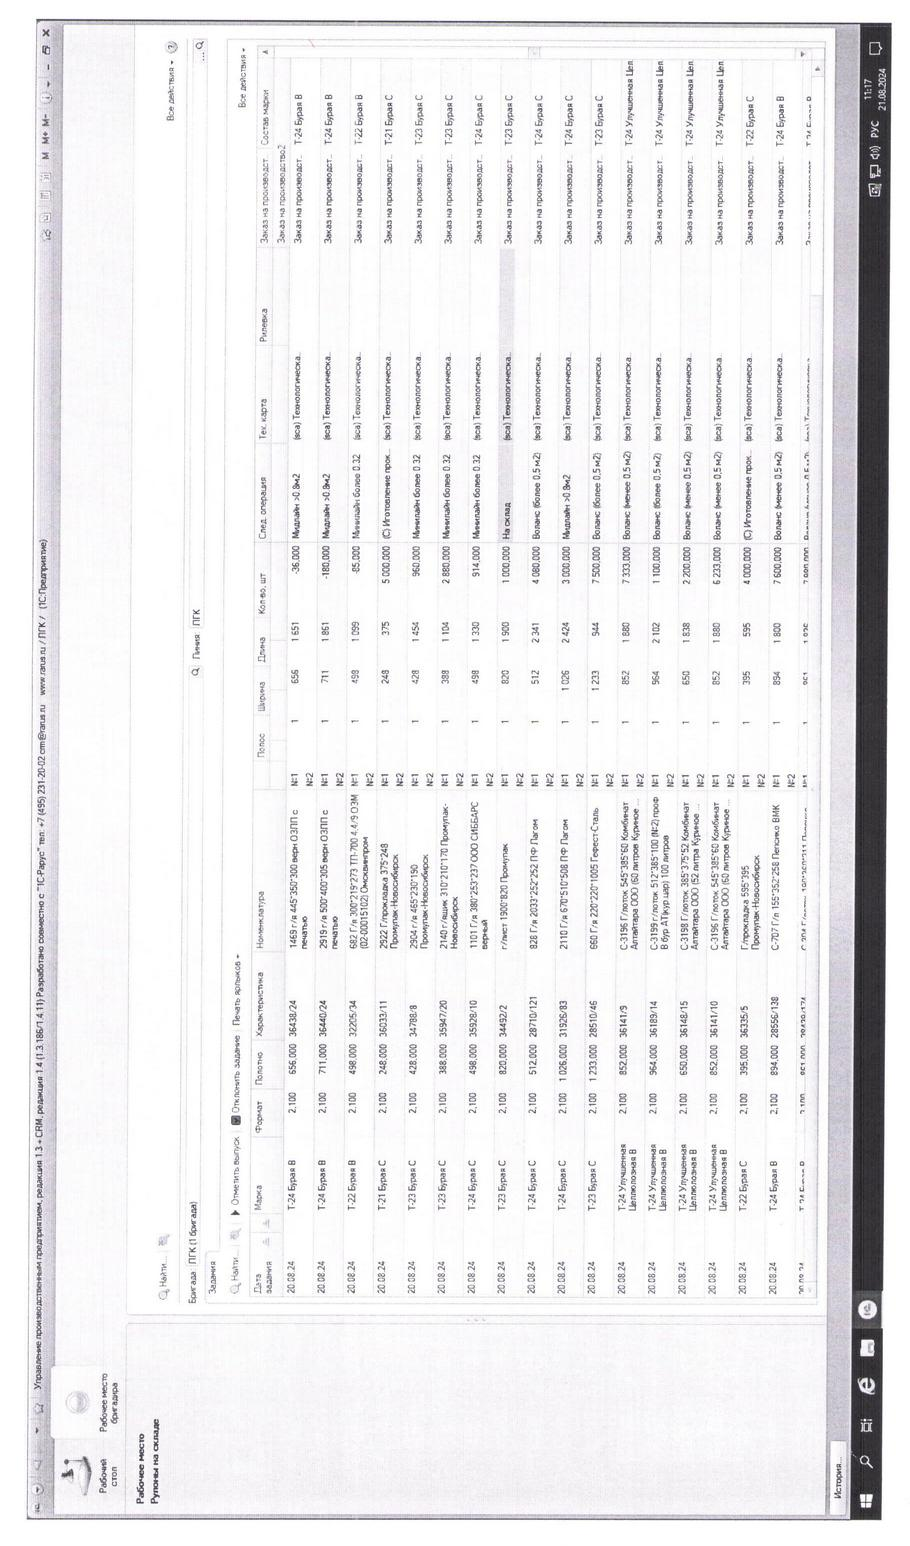
\includegraphics[height=0.8\textheight, width=\textwidth, keepaspectratio]{Pics/d19.jpg}
% \end{center}
%   \caption{Оборотная ведомость по материалам}
%   \label{pic:d19}
% \end{figure}


% \begin{figure}
% \begin{center}
%   \includegraphics[height=0.94\textheight, width=0.94\textwidth, keepaspectratio]{Pics/a7.jpg}
% \end{center}
%   \caption{Отчет по краске в системе}
%   \label{pic:a7}
% \end{figure}

%
\clearpage
\ifx \notincludehead\undefined
\normalsize
\end{document}
\fi